\chapter{PROJECT PLANNING}
\label{sec:project_planning}

\section{Work Breakdown Structure (WBS)}

The wbs is shown in \fref{fig:wbs}. It is divided into subteams with a "general" title for all system-wide tasks.

\begin{center}
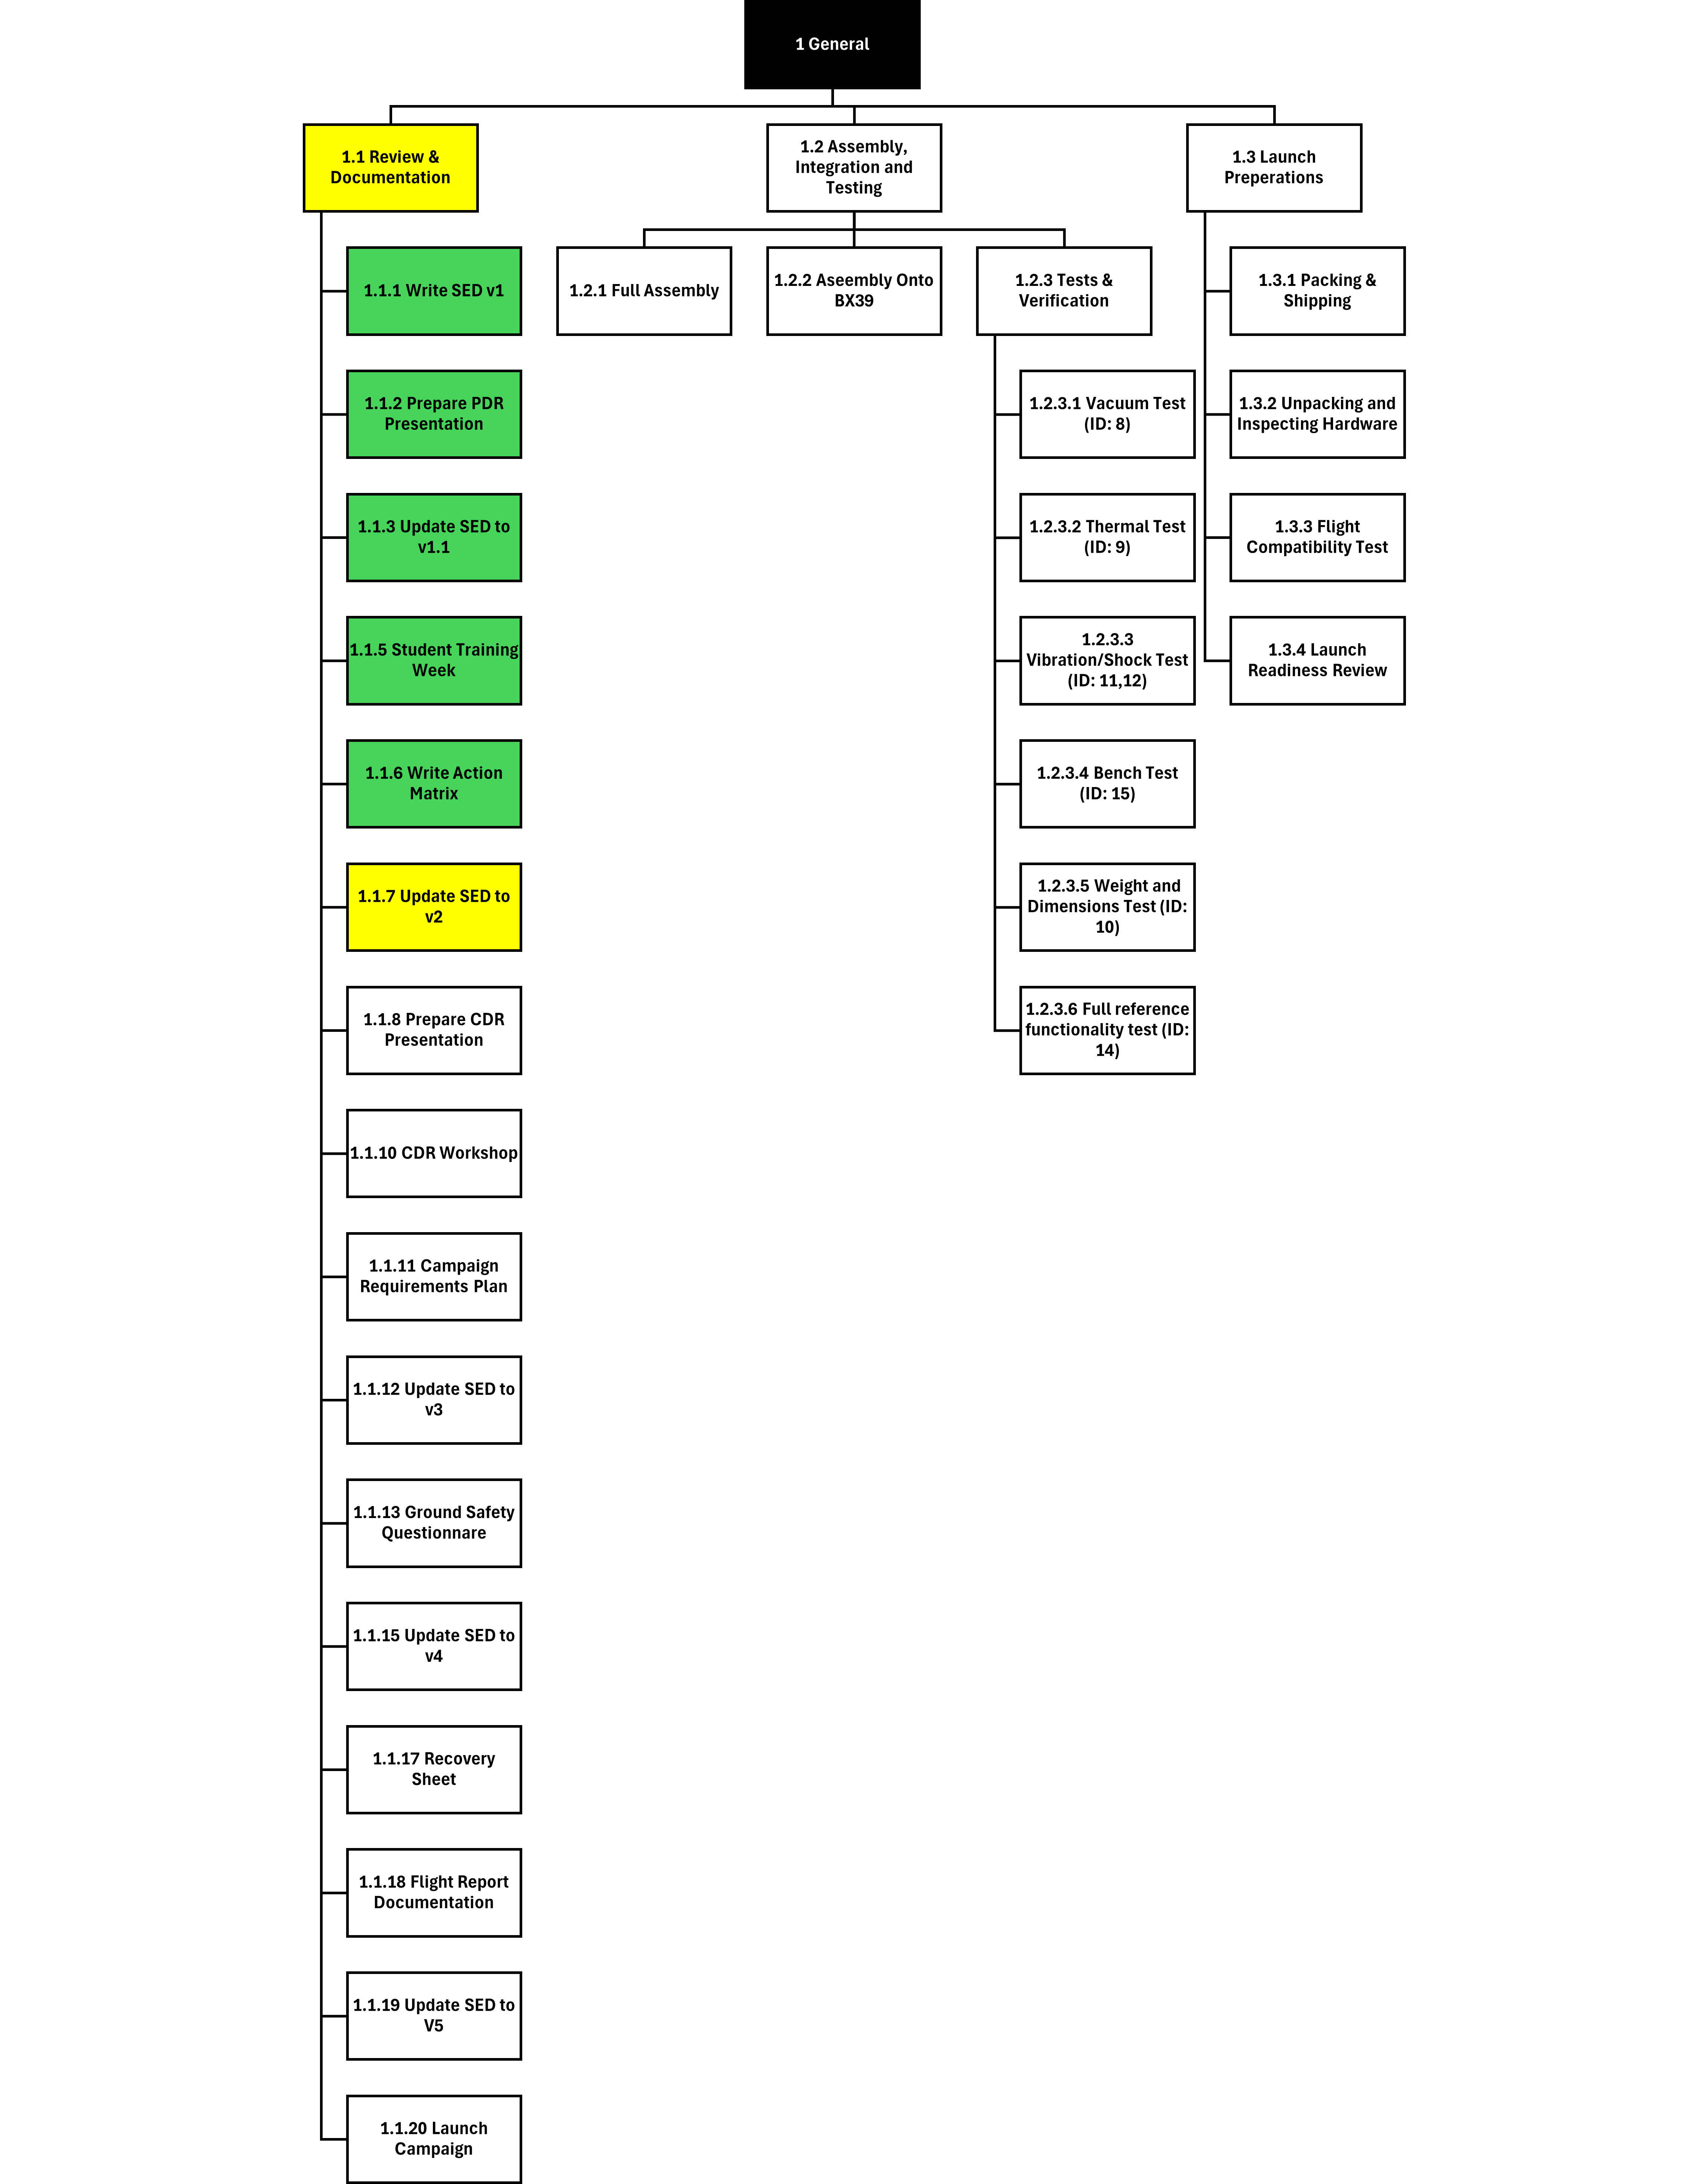
\includegraphics[width=0.8\textwidth]{0_images/figures/wbs_general.png}

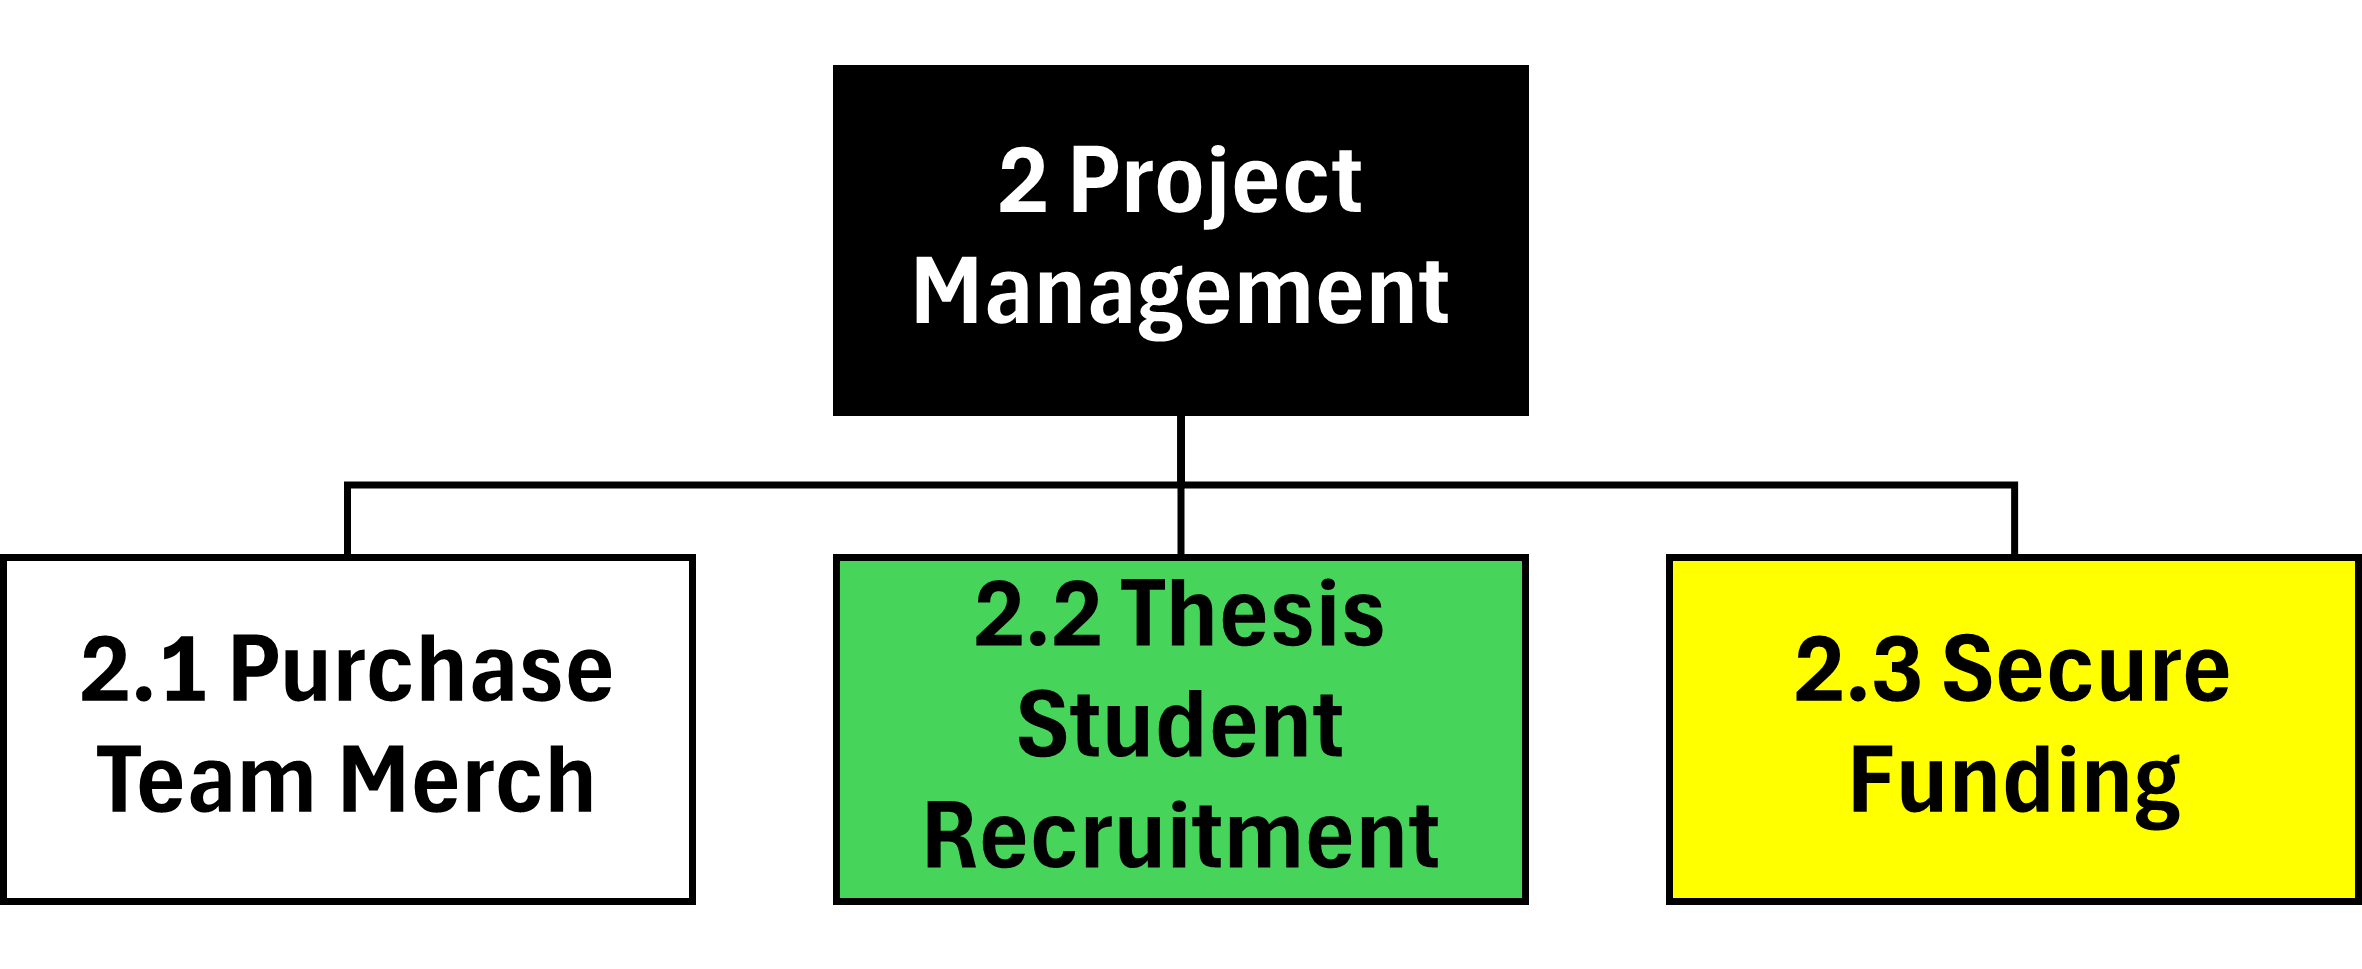
\includegraphics[width=0.8\textwidth]{0_images/figures/wbs_manegerial.png}

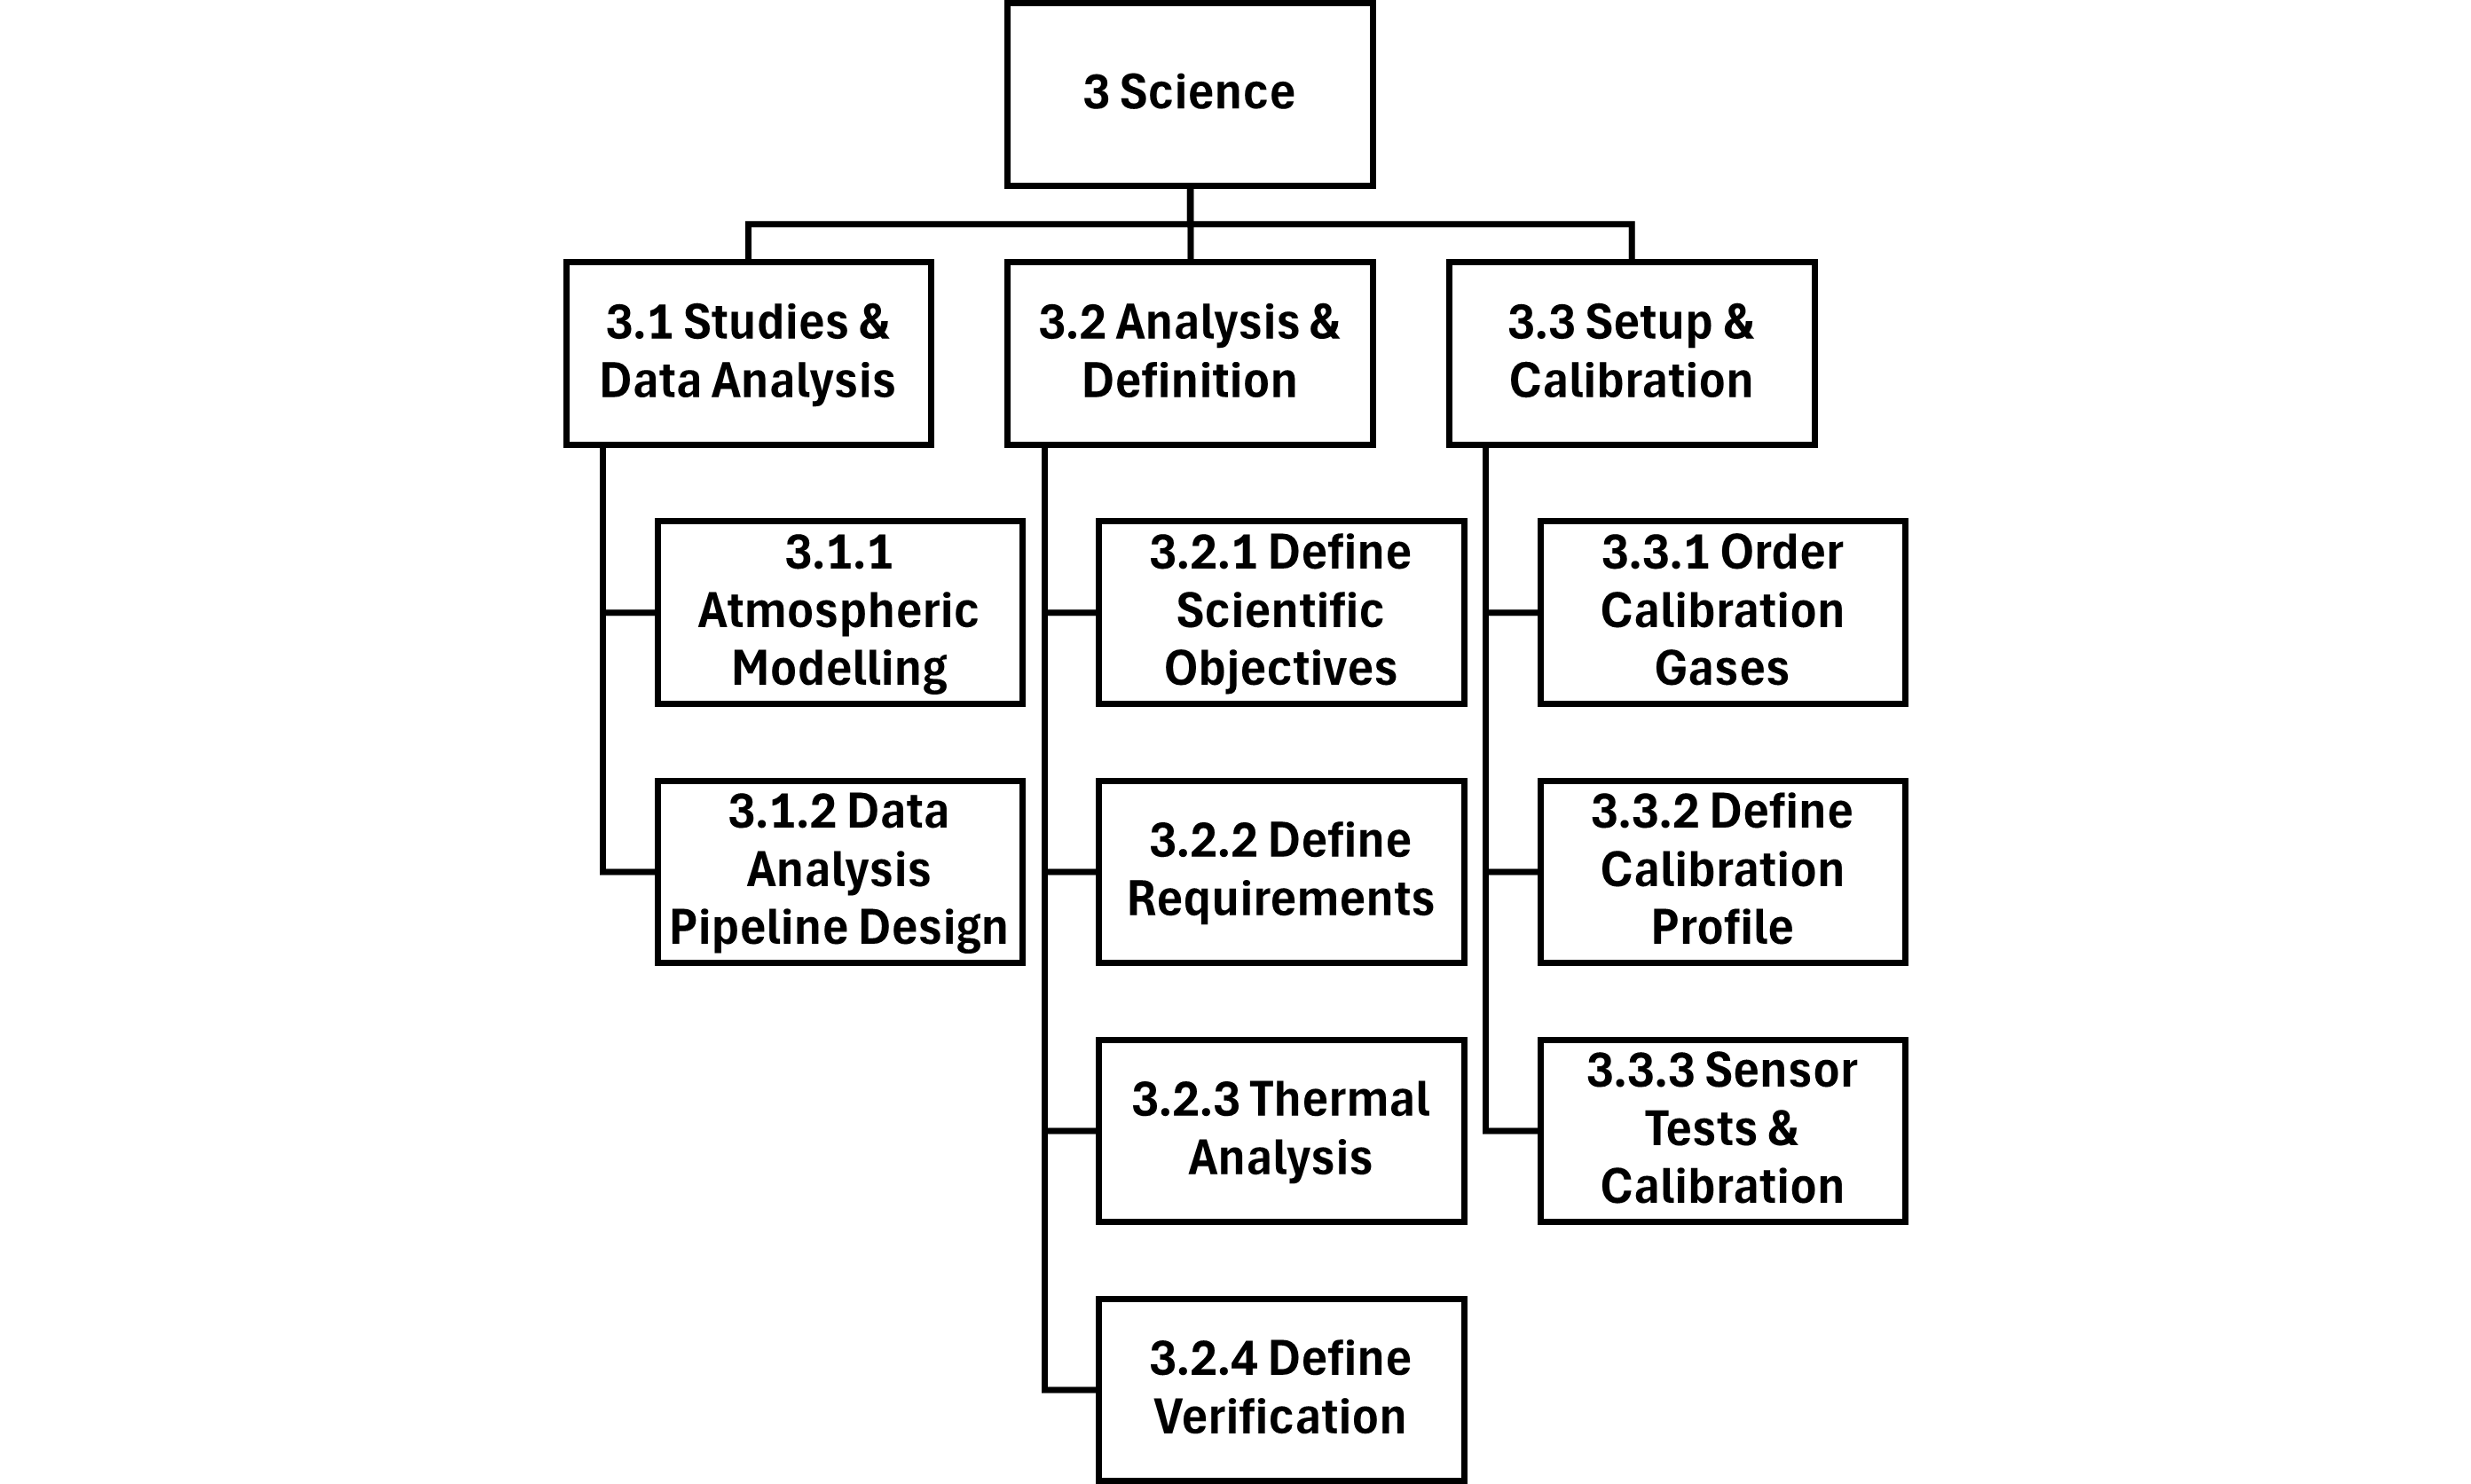
\includegraphics[width=0.8\textwidth]{0_images/figures/wbs_science.png}

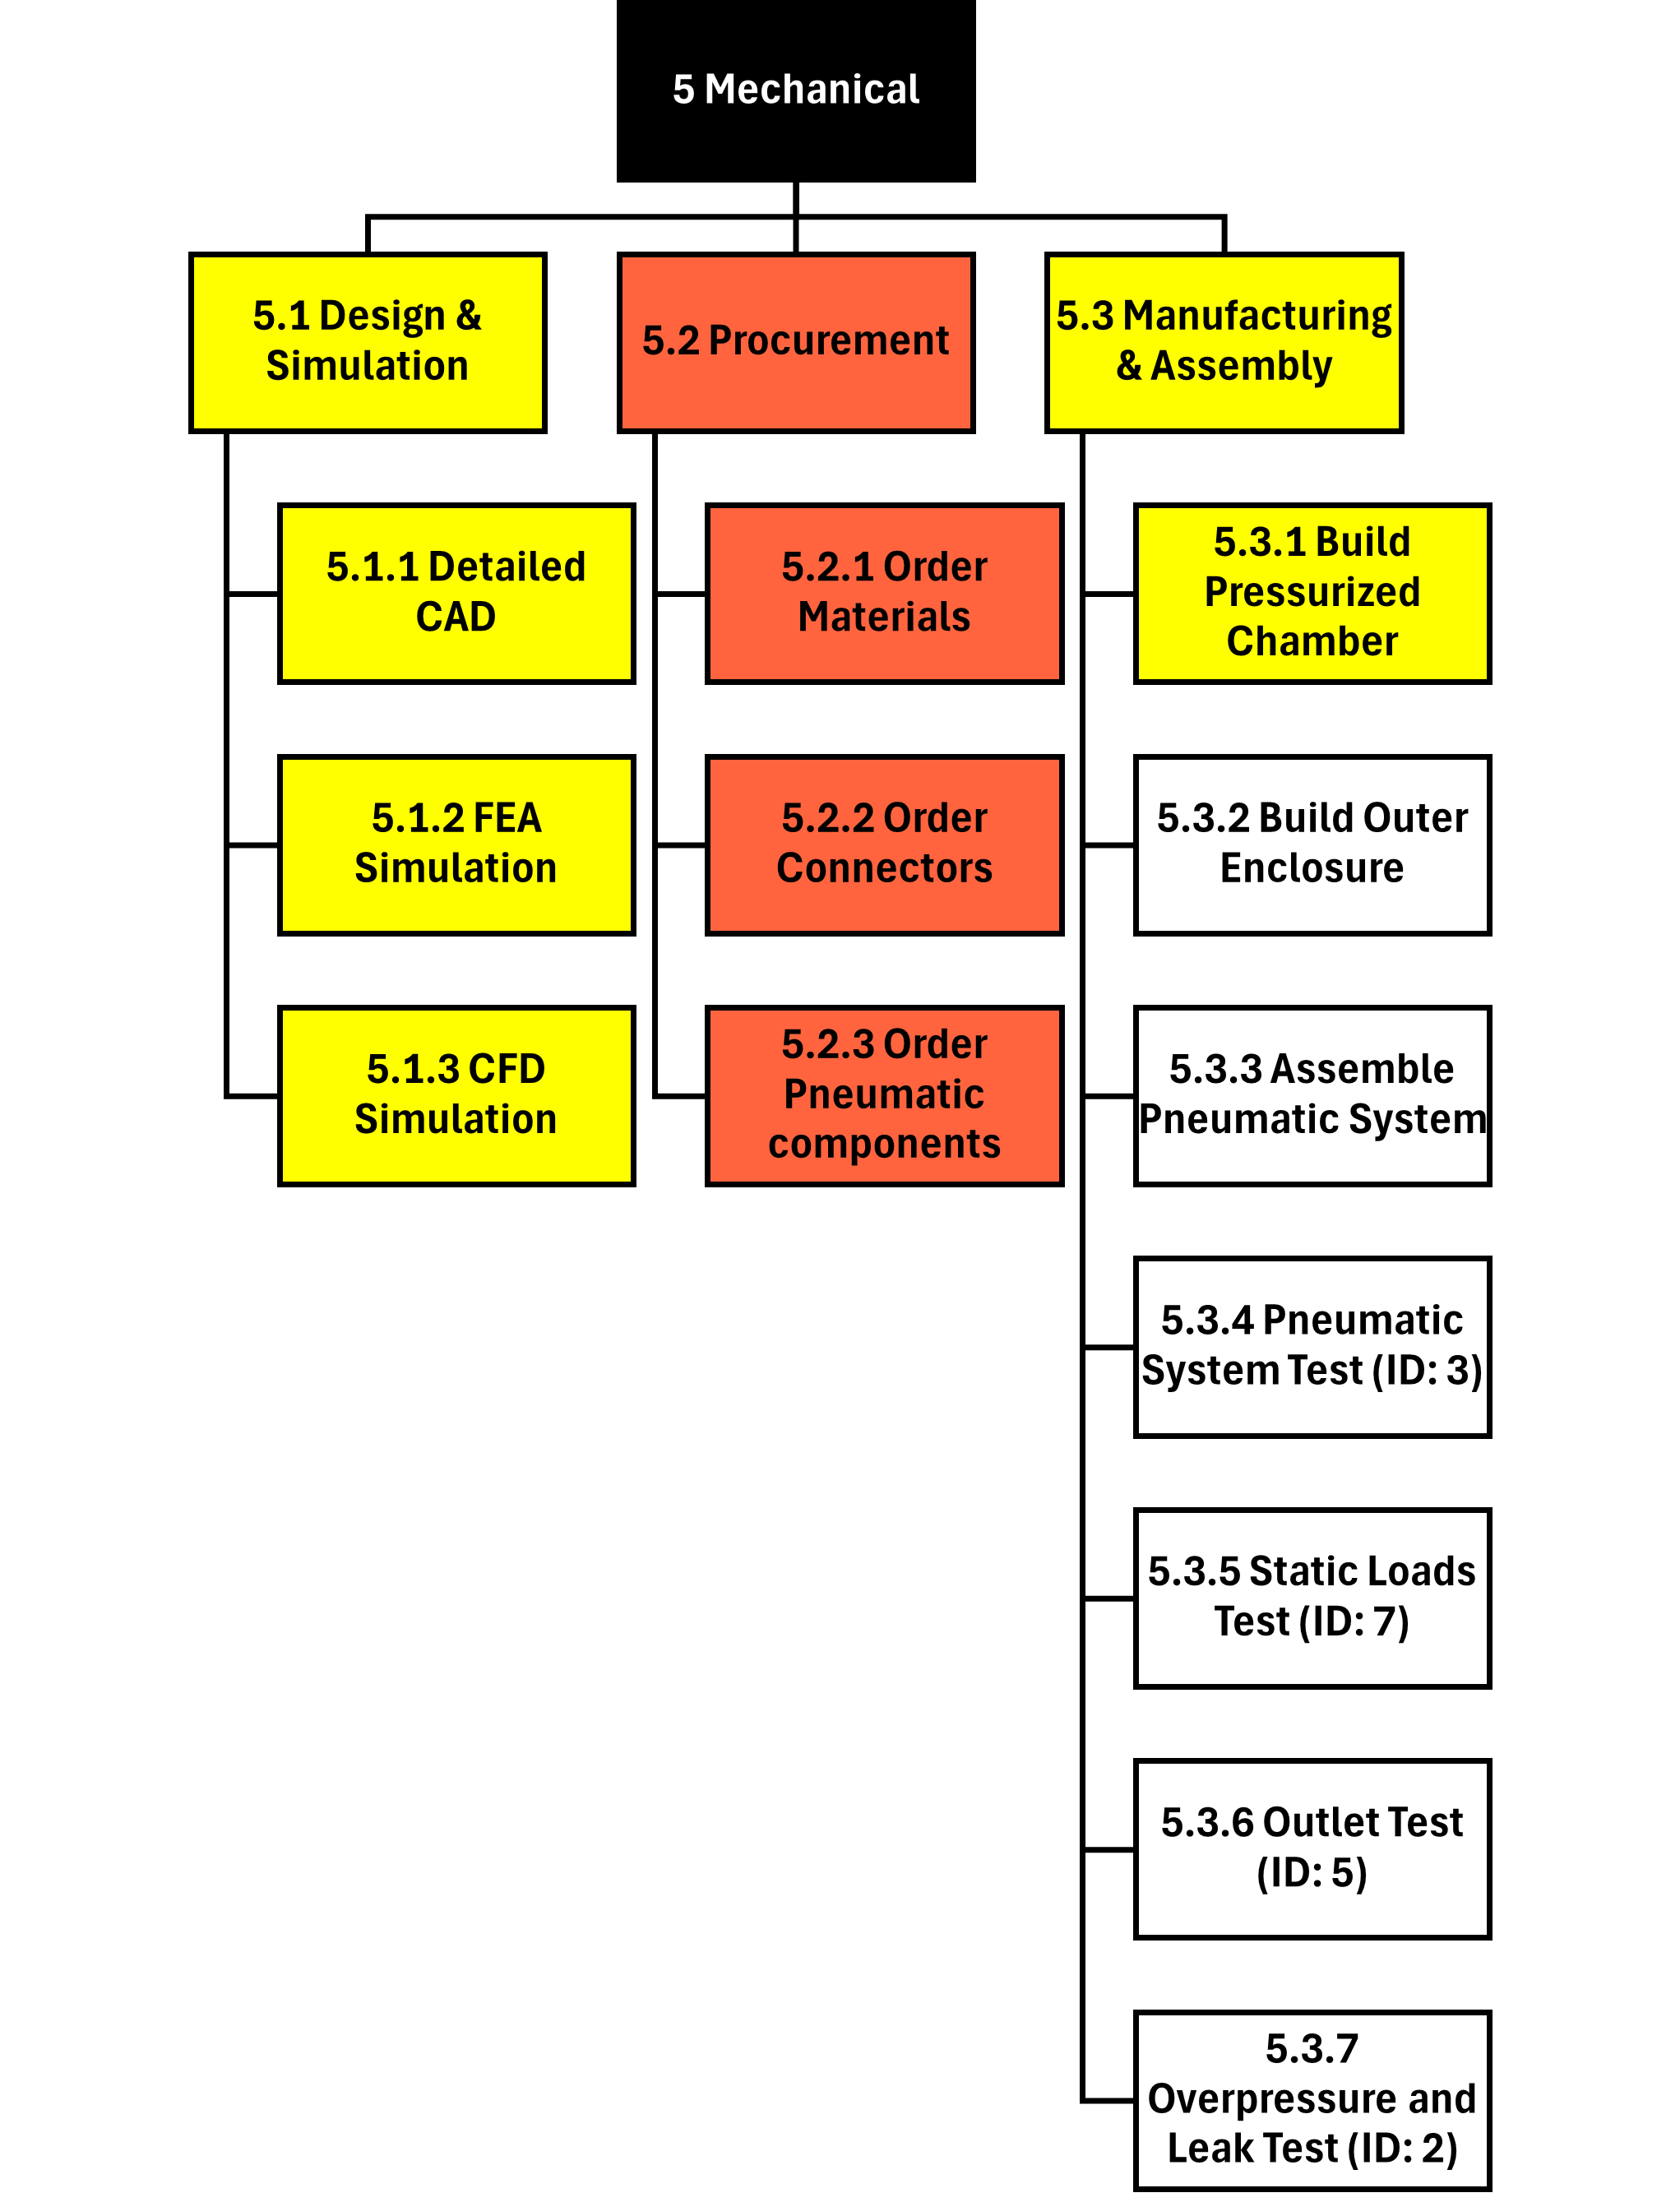
\includegraphics[width=0.8\textwidth]{0_images/figures/wbs_mechanical.png}

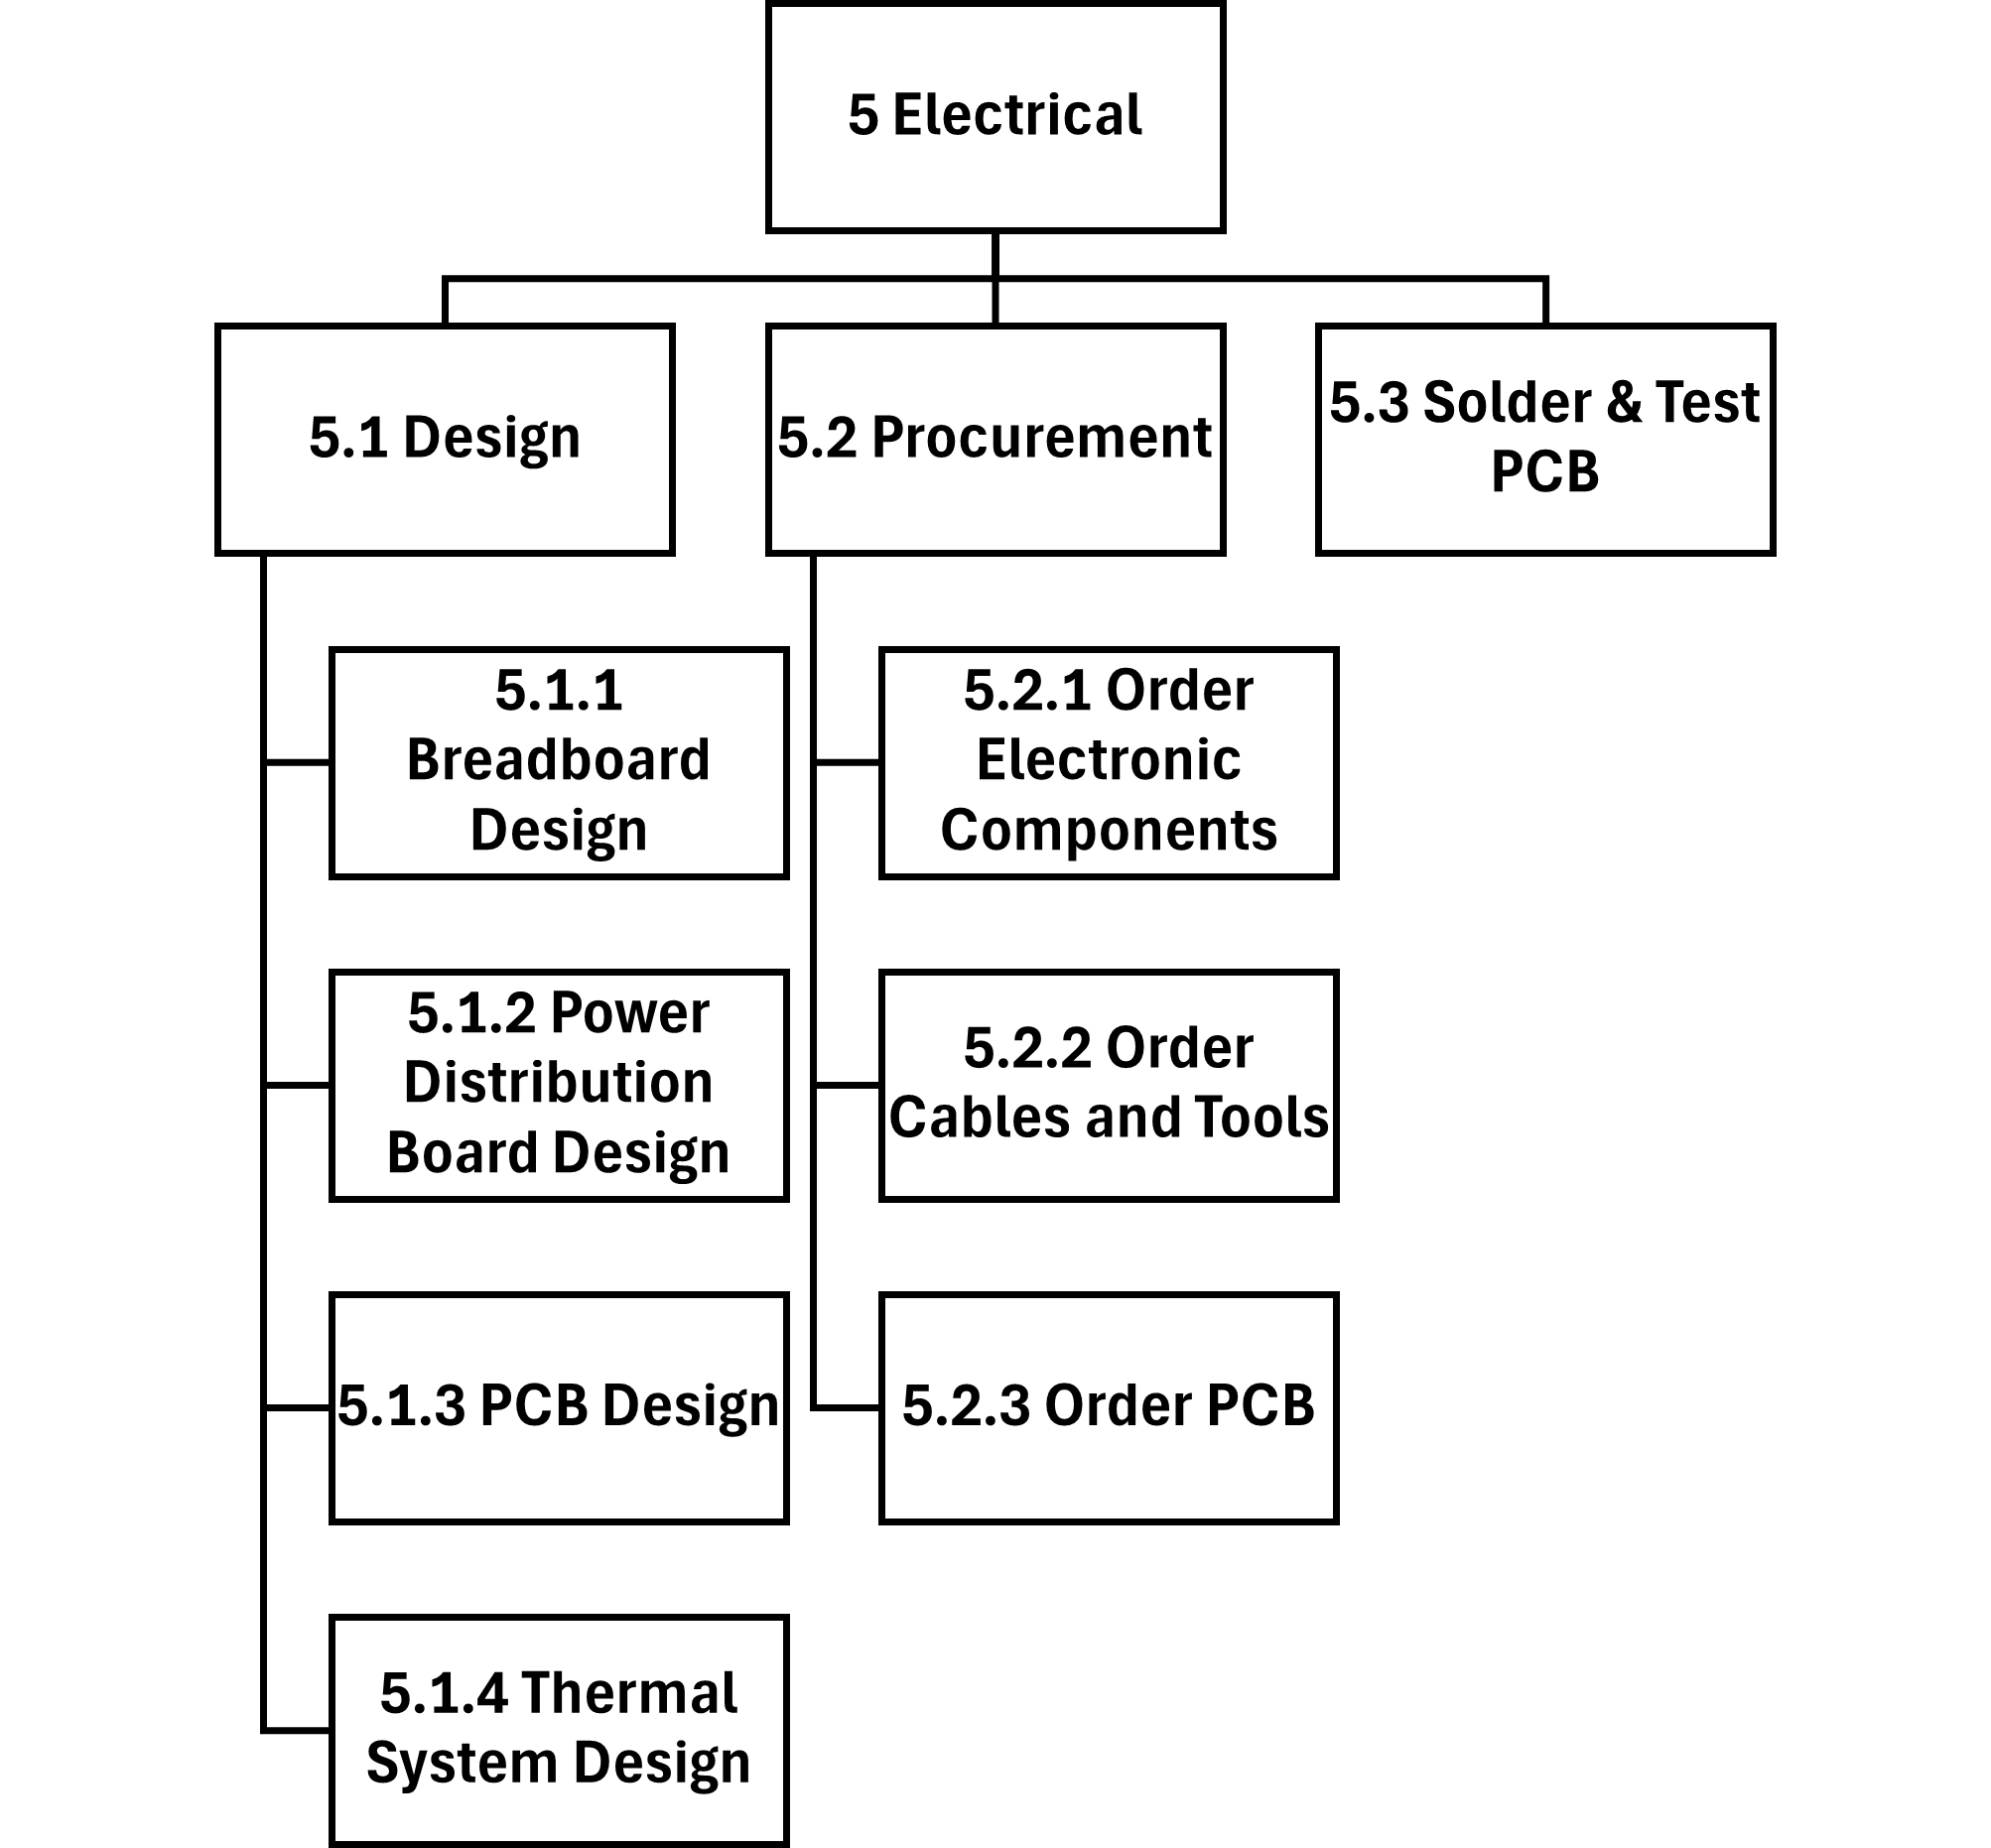
\includegraphics[width=0.8\textwidth]{0_images/figures/wbs_electrical.png}

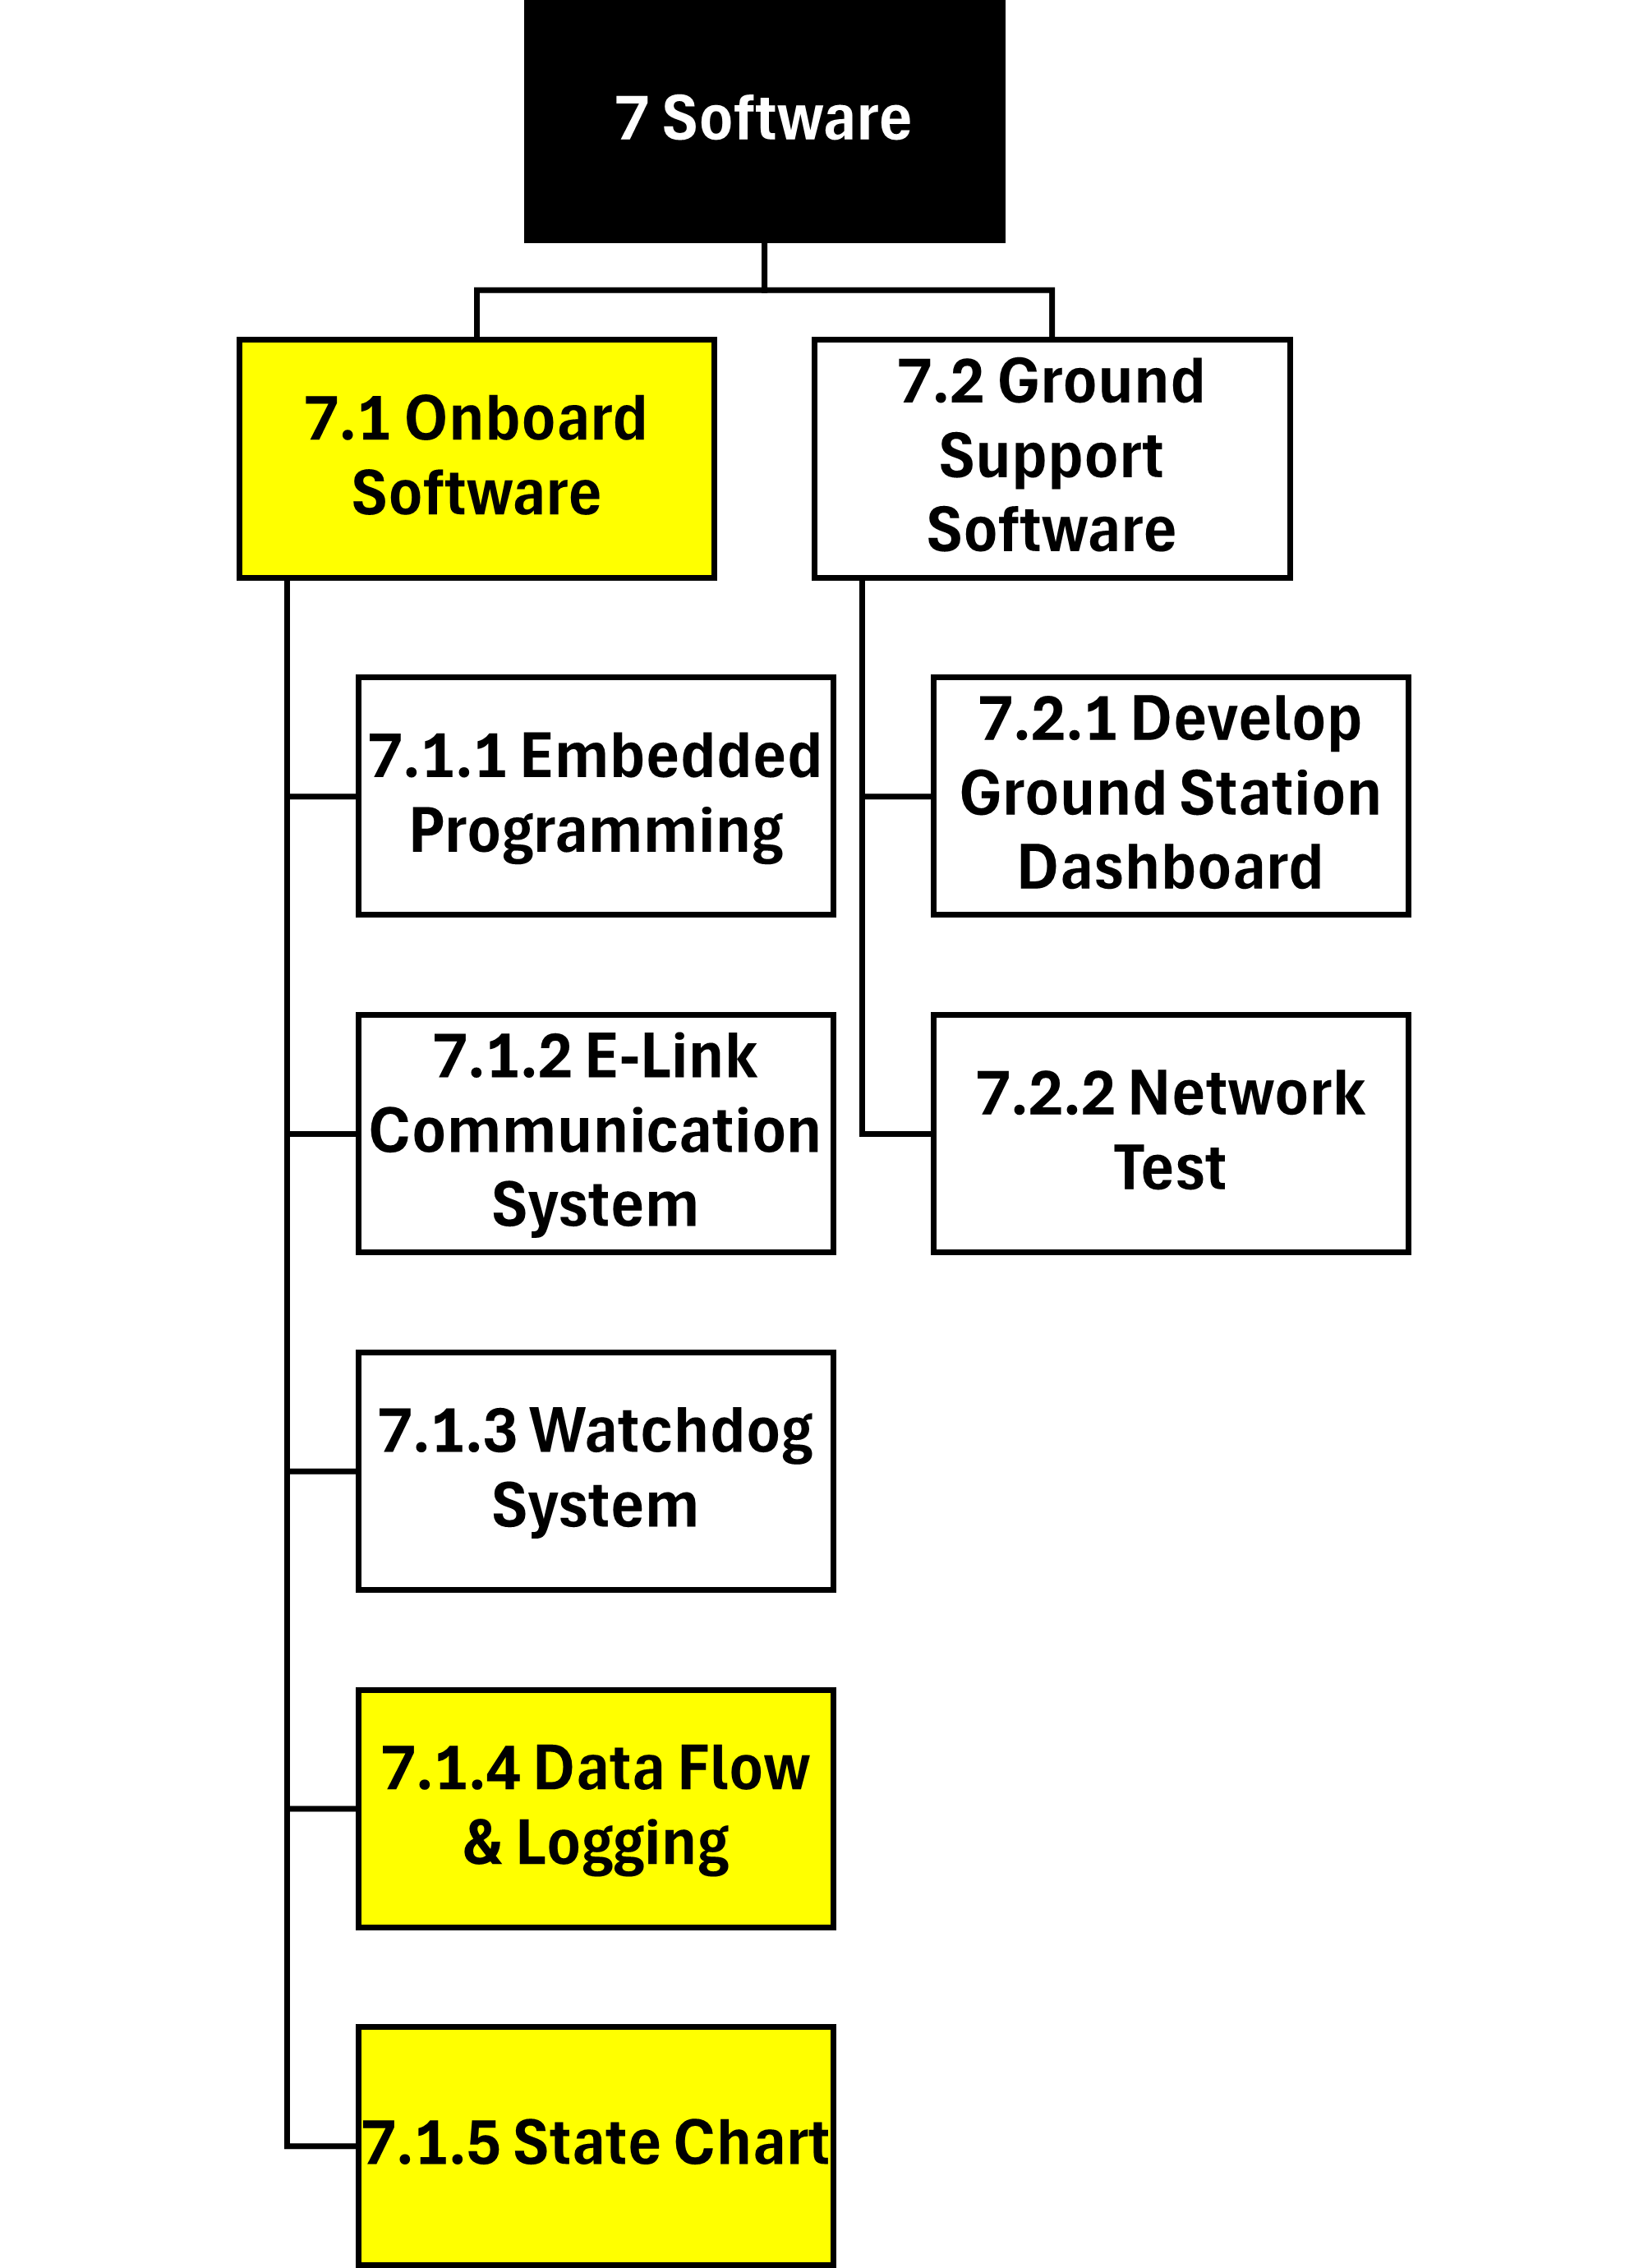
\includegraphics[width=0.8\textwidth]{0_images/figures/wbs_software.png}

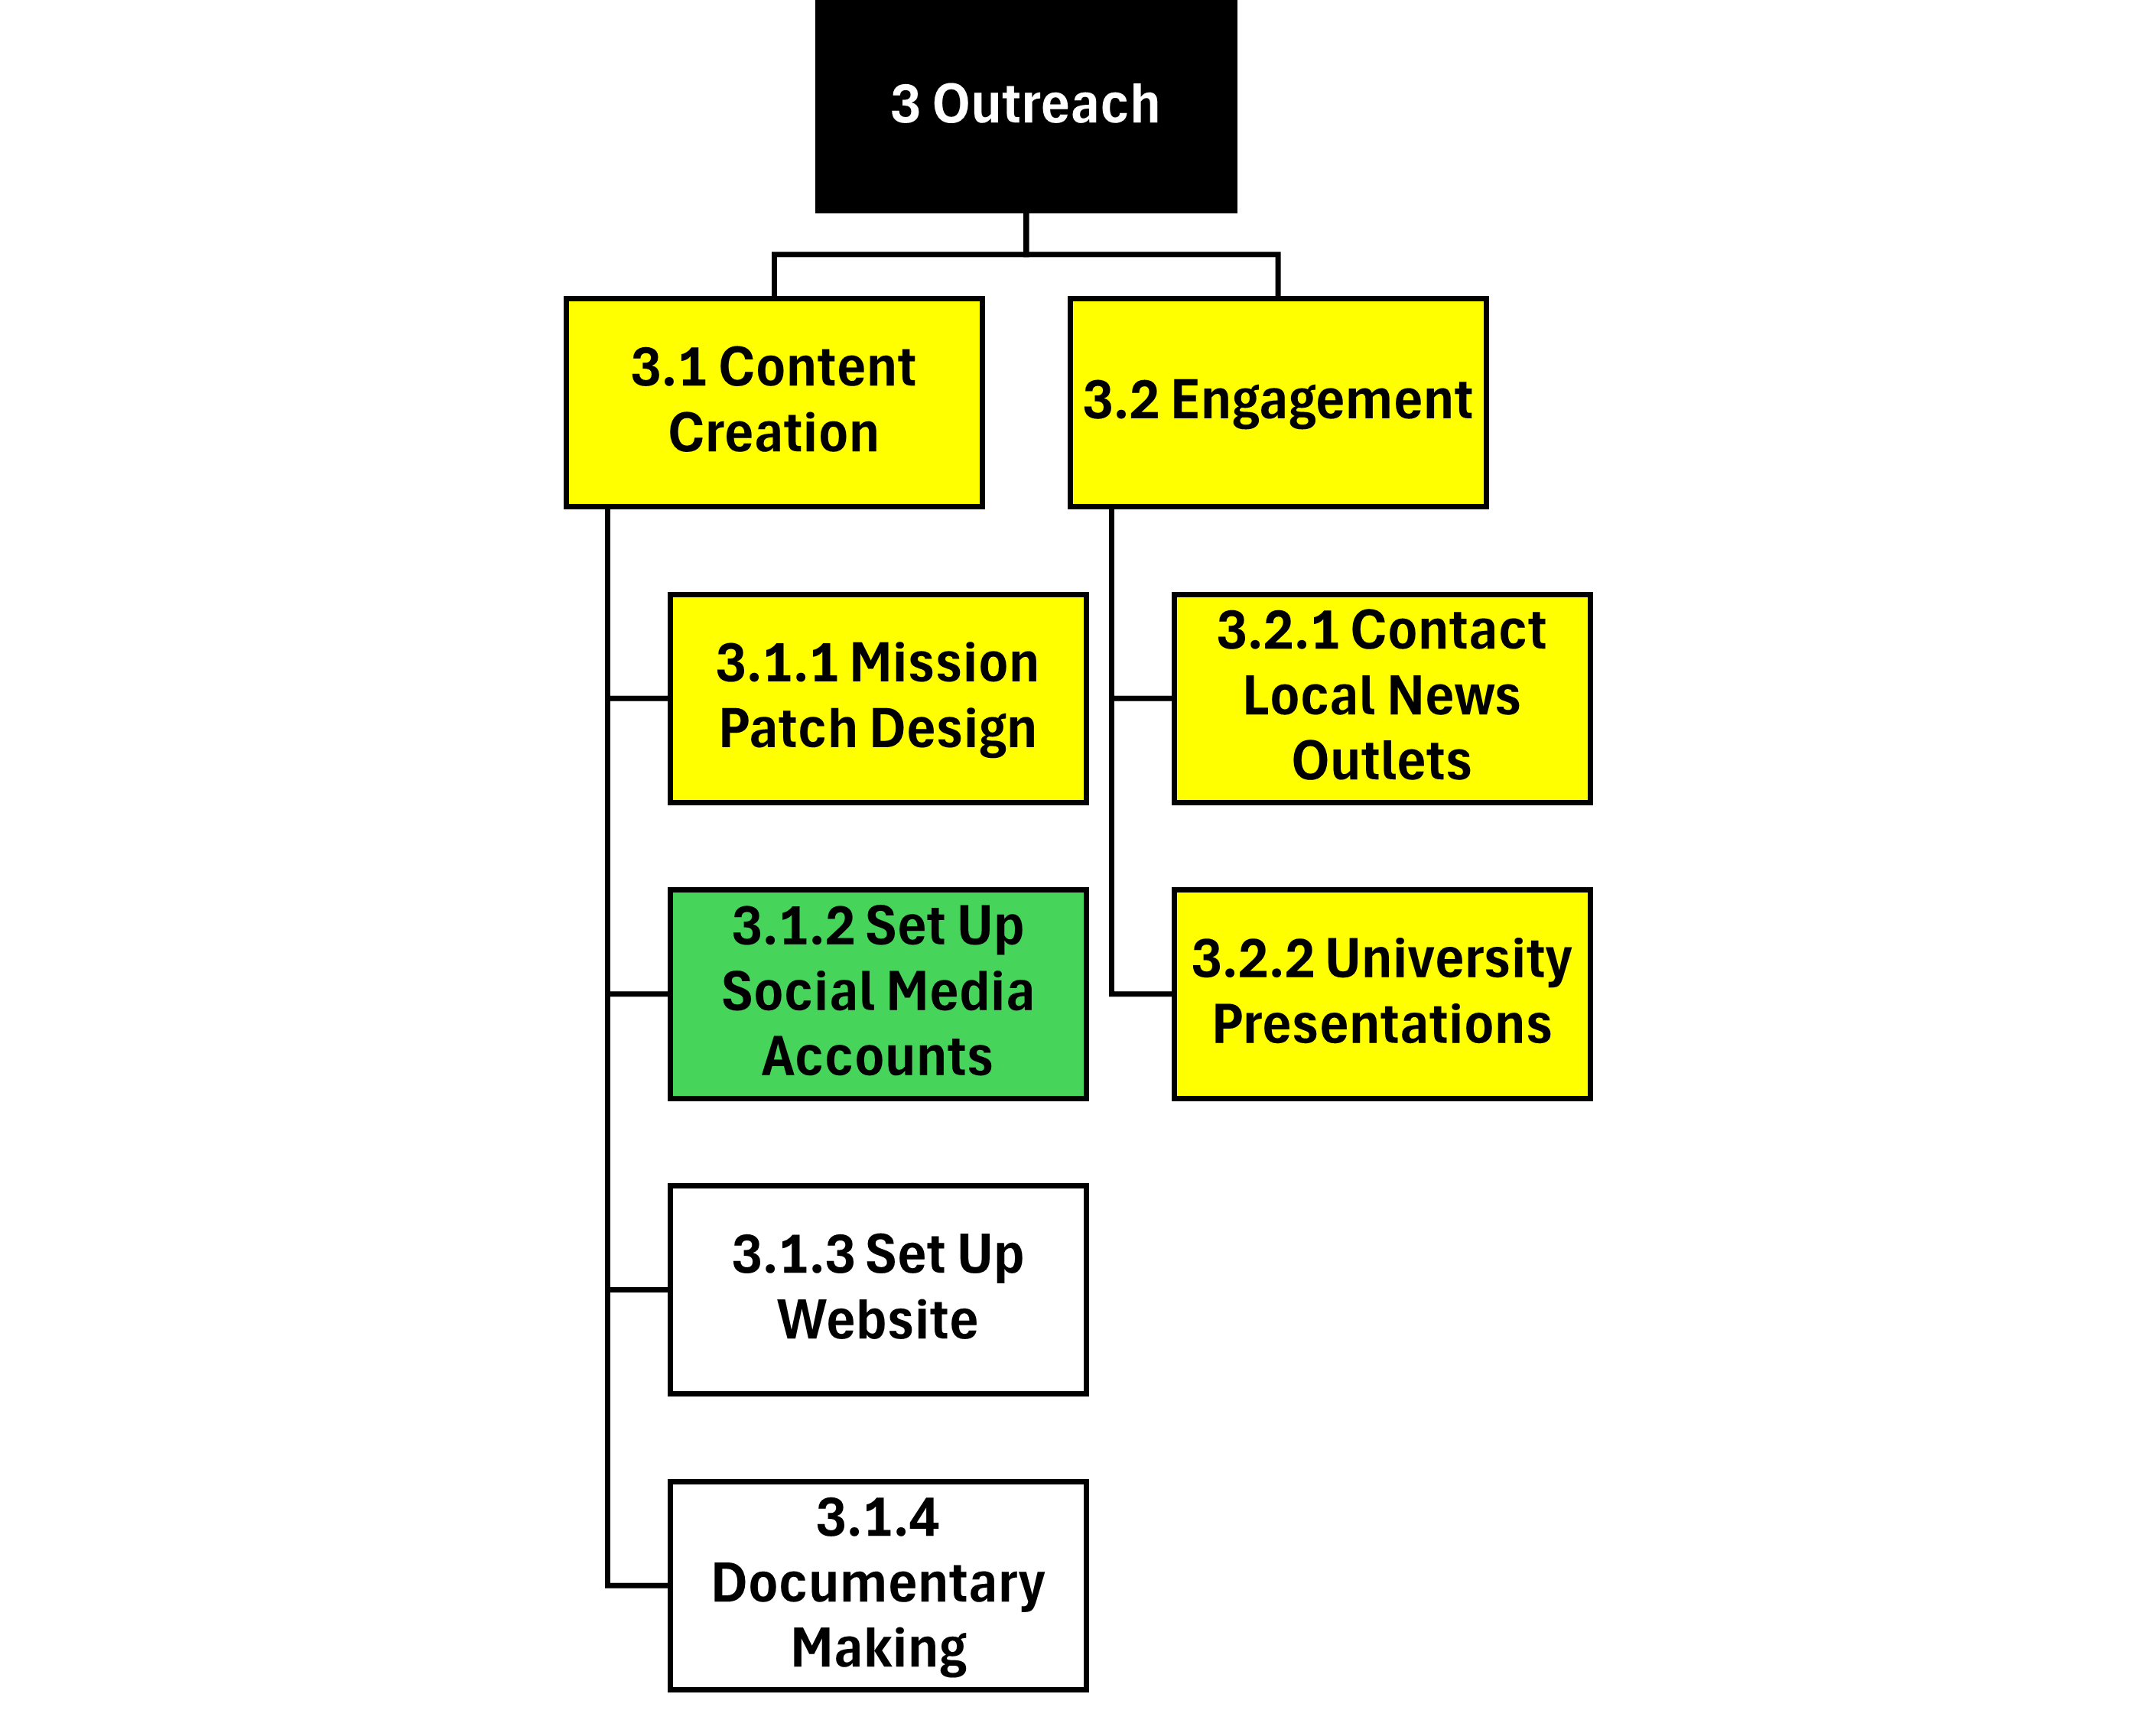
\includegraphics[width=0.8\textwidth]{0_images/figures/wbs_outreach.png}

\captionof{figure}{WBS for all subsystems and general tasks}
\label{fig:wbs}
\end{center}

% %%%%%%%%%%%%%%%%%%%%%%%%%%%%%%%%%%%%%%%%%%%%%%%%%%%%%%%%%%%%%%%%%%%%%%%%%%%%%%%
\section{Schedule}

A Gantt chart has been made to visualize the work to be done and the duration of specific tasks. It was divided into the different subteams in addition to a system wide \gls{ait}. The Gantt chart is shown in \fref{fig:gantt}, with the critical path highlighted in red.

The critical path is Define Scientific Objectives - Define Requirements - Order Materials - Build Pressurized Chamber. This demonstrates the importance of the pressurized chamber on the whole experiment and thus the project planning.

\gls{mirage} team members have declared their availability per week throughout the project duration, so that certain people were assigned different tasks.

OnlineGantt was used to manage scheduling and assigning the tasks, whereas Discord is used for communications within the team.

\begin{figure*}[htbp]
    \centering
    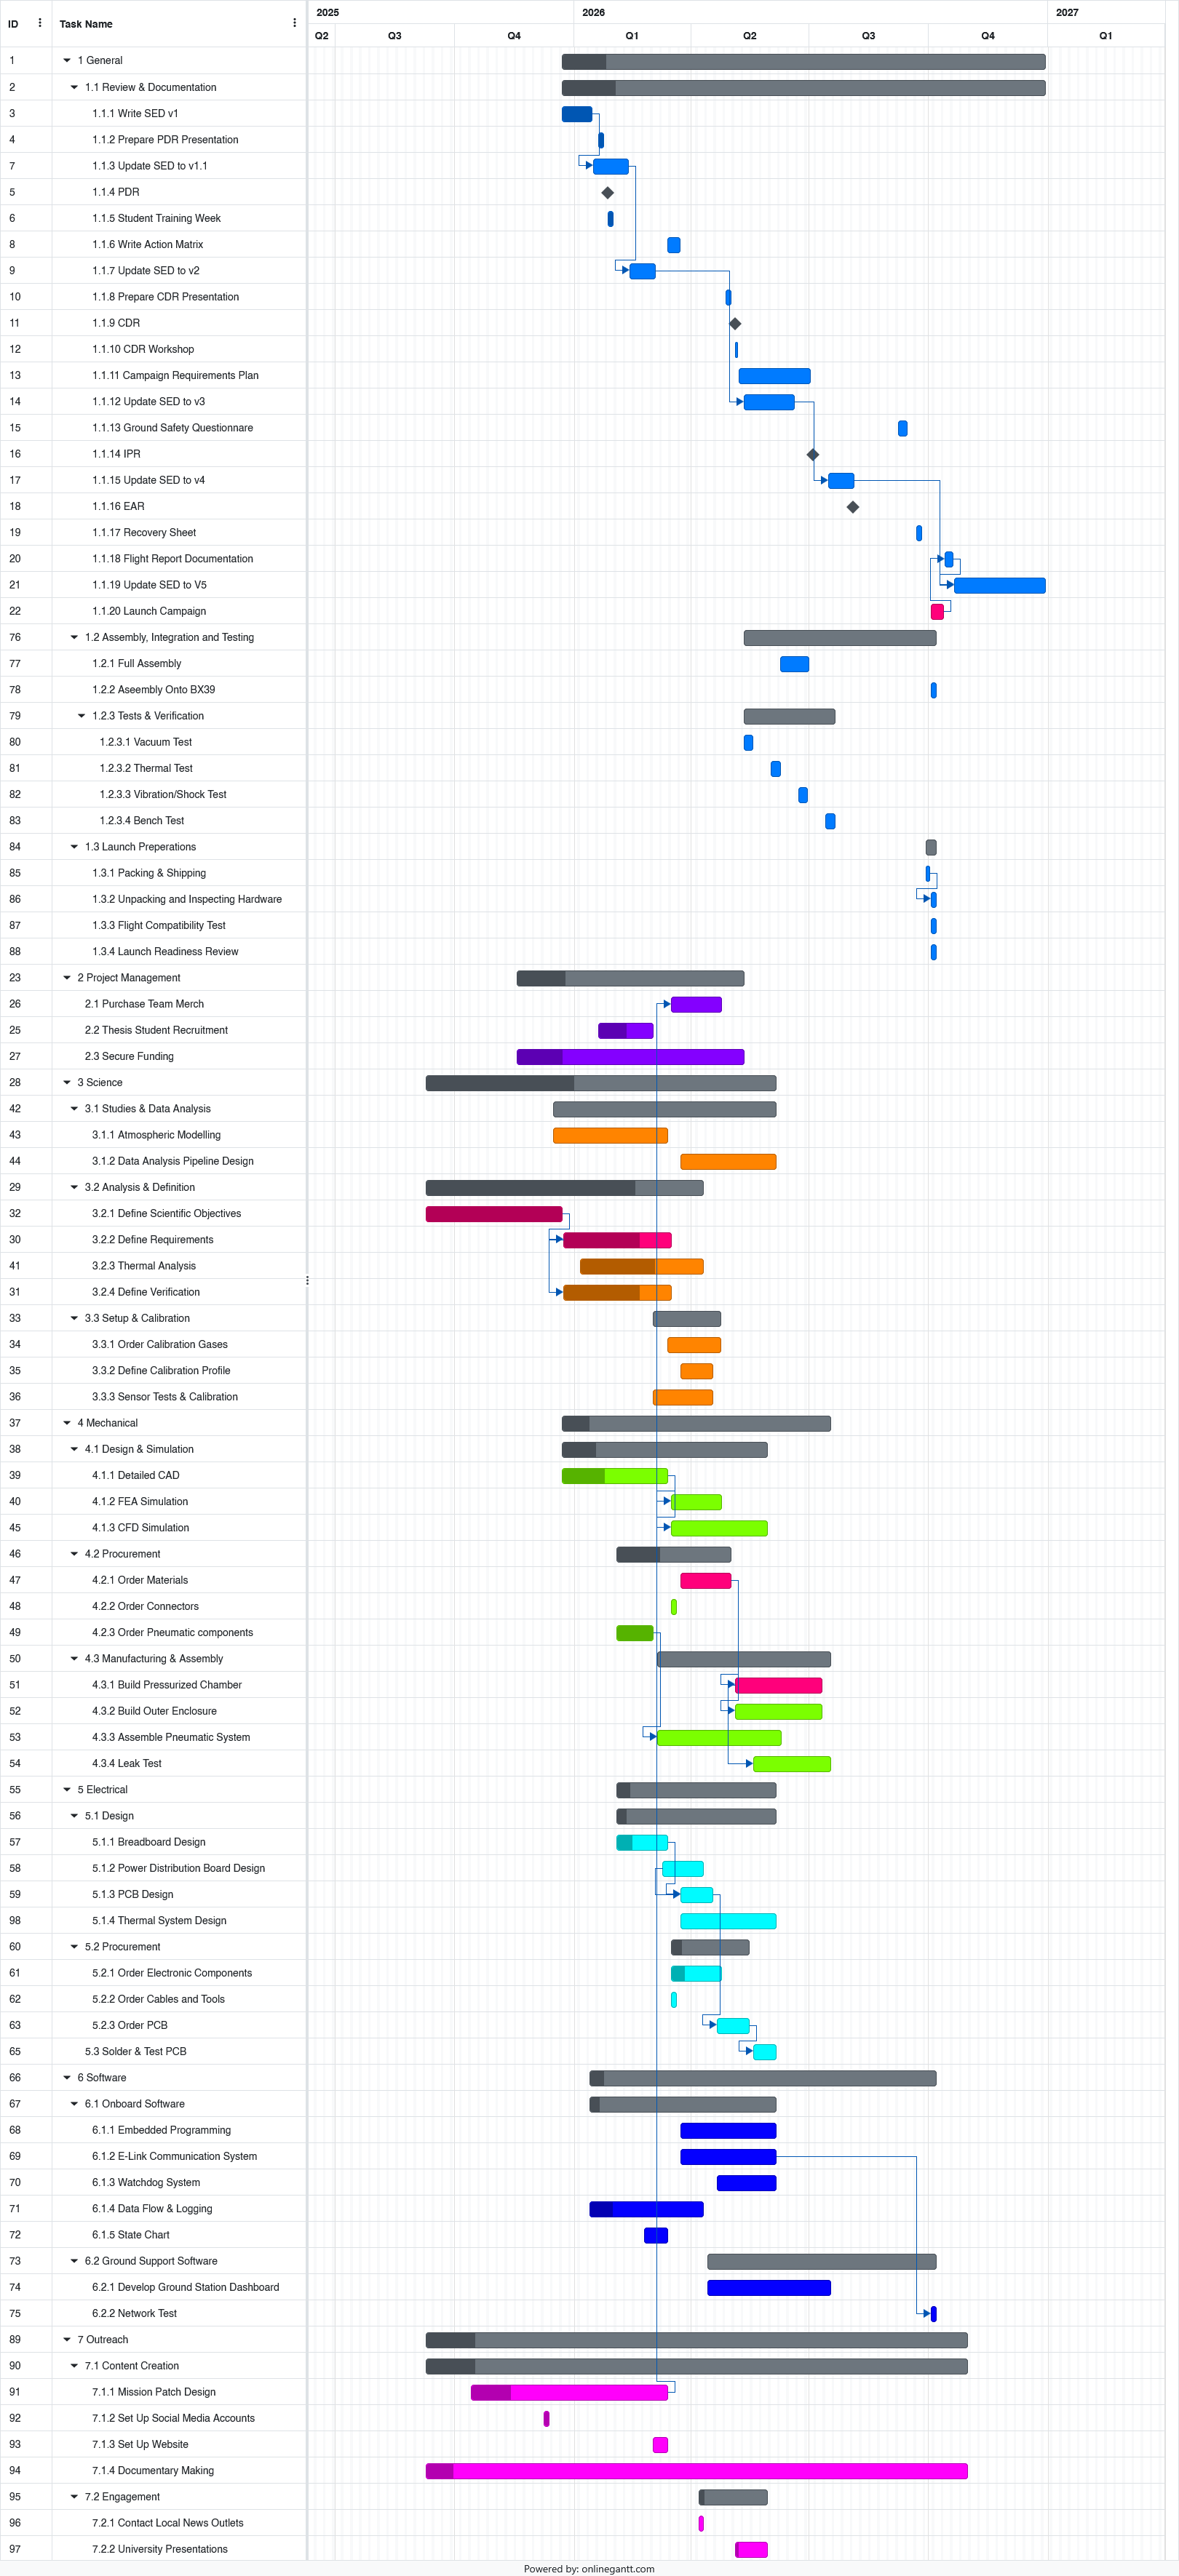
\includegraphics[height=22cm]{0_images/figures/gantt.png}
    \caption{Gantt chart for the MIRAGE experiment. Critical path is hightlighted in red.}
    \label{fig:gantt}
\end{figure*}

% %%%%%%%%%%%%%%%%%%%%%%%%%%%%%%%%%%%%%%%%%%%%%%%%%%%%%%%%%%%%%%%%%%%%%%%%%%%%%%%
\section{Resources}

\gls{mirage} is a project conducted by the RiseUpp association, which is under the umbrella of Astronomisk Ungdom. The RiseUpp association has a dedicated outreach team working on finding sponsors. Currently \gls{mirage} is the only project RiseUpp is working on, therefore a majority of this budget will go to \gls{mirage}.

As part of Astronomisk Ungdom, RiseUpp get annually 2000 SEK and 20 SEK per member. RiseUpp aims to be an association at Uppsala university that gathers all students interested in space, hosts events such as lunch lectures, and participate in programmes like Rexus Bexus.

The \gls{mirage} project will consist mostly of students working on their thesis, therefore Uppsala university covers costs up to 1000 SEK per student. In addition, through the team's supervisor, Uwe Zimmermann, access to a laboratory with the necessary tools and a vacuum chamber for testing is given. Uppsala university also hosts the Swedish Institute for Space Physics (Institutet för Rymdfysik), which has a thermal chamber that will be used for testing.

RiseUpp has an agreement with the Swedish company SenseAir AB, in which SenseAir AB has provided a brand new K96 sensor, a used K96 sensor for testing, \gls{ir} lamps (which are a critical part of the K96 sensor) and will provide extra gas sensors if needed.

In addition, the sensor calibrations will be done in collaboration with the Norunda weather stations; who will provide gas samples and a Picarro gas analyzer for reference.

The gas pumps and the compressor are purchased and received, which is another crucial component to the mission.

% %%%%%%%%%%%%%%%%%%%%%%%%%%%%%%%%%%%%%%%%%%%%%%%%%%%%%%%%%%%%%%%%%%%%%%%%%%%%%%%
\subsection{Workforce}

The workforce consists of voluntary and thesis students. Voluntary students spend around 10 hours a week and will be the main workforce until March, they do this voluntarily and will be the core team members. Thesis students are recruited to begin working on the project from March, they will work in project groups under the supervision of the team's supervisor, Associate Professor Uwe Zimmermann, and will get credited for the work. The thesis project will be 15 credits, and the students are expected to work full-time on the project from 23rd of March until the 5th of June.

More information about the thesis projects is shown in \tref{tab:thesis}. Thesis students will not directly write into the \gls{sed} but they will write their own university reports.

One task for the voluntary students is to mentor and follow up with the thesis students. The voluntary students cover all subteams and will act as the interface between the thesis projects and the \gls{mirage} project.

There are weekly meetings for the whole team in which the core team members will follow up closely with the thesis projects and update on the progress, in addition to an extra subteam meeting each week to work on given tasks and plan the next steps. Thesis students will have the chance, and be encouraged, to continue working on the project voluntarily.

\begin{table}[htbp]
\centering
\caption{Thesis Projects Overview}
\label{tab:thesis}
\begin{tabular}{|l|L{3.5cm}|L{5.5cm}|}
\hline
\textbf{Project Number} & \textbf{Project Name} & \textbf{Project Description} \\ \hline

1 & Finite Element Analysis (FEA) and Computational Fluid Dynamics (CFD) 
& Finite Element Analysis (FEA) of temperature and stress \& Computational Fluid Dynamics (CFD) to analyze airflow. 
\\ \hline

2 & PCB Design and Embedded Programming 
& Printed circuit board (PCB) design, component selection, and embedded programming. 
\\ \hline

3 & Pressurized Gas Sensing Compartment 
& Design and assembly of a pressurized gas sensing experiment compartment. 
 \\ \hline

4 & Data Analysis Pipeline 
& Data analysis pipeline programming. 
 \\ \hline

5 & NDIR Sensor Testing and Calibration 
& Sensor testing and calibration of an NDIR gas sensor for stratospheric pressure and temperature conditions. 
 \\ \hline

6 & Thermal System Design 
& Thermal system design. 
 \\ \hline

7 & ECSS-Based Material Selection 
& Material selections in accordance with ECSS guidelines for a leakage-free and heat-resistant compartment. 
 \\ \hline

8 & Power Distribution Board Design 
& Power distribution board design. 
\\ \hline

\end{tabular}
\end{table}

In addition to the \gls{mirage} workforce, there is the RiseUpp board which will ensure the consistency of the team and assemble a team for the next Rexus Bexus cycles.
\clearpage

% %%%%%%%%%%%%%%%%%%%%%%%%%%%%%%%%%%%%%%%%%%%%%%%%%%%%%%%%%%%%%%%%%%%%%%%%%%%%%%%
\subsection{Budget}

The estimated total budget of the experiment \emph{parts} without the K96 sensor is 6089 SEK, and with a 15\% buffer is 7000 SEK ($\approx$ 650 EUR). The K96 sensor, which was sponsored, is not commercially available and was estimated to be 5000 SEK; making the total cost of the experiment around 1200 EUR. Additional managerial costs like outreach and travel expenses lead to a sum of approximately 85000 SEK ($\approx$ 8000 EUR).

For the hardware, \gls{mirage} was sponsored by SenseAir AB and received 2 K96 sensors; one for testing and one for use. Additionally, the pumps and the compressor were ordered.

All of the hardware costs can be covered by the money given through Uppsala university for the thesis projects, however \gls{mirage} aims to find external sponsors for additional outreach budget. Additional material such as cables, screws, RTCs and small microcontrollers are available for the team in the designated lab at Uppsala university and is provided; they were not added to the total cost.

\begin{longtable}{p{3cm}p{1.7cm}p{1.5cm}p{3cm}p{5cm}}
\caption{Budget Breakdown}
\label{tab:budget}\\

\toprule
\textbf{Cost Name} & \textbf{Quantity} &
\textbf{Unit Price (SEK)} &  \textbf{Status} & \textbf{Description} \\
\midrule
\endfirsthead

\multicolumn{5}{c}{\tablename\ \thetable\ -- \textit{Continued from previous page}}\\
\toprule
\textbf{Cost Name} & \textbf{Quantity} &
\textbf{Unit Price (SEK)} &  \textbf{Status} & \textbf{Description} \\
\midrule
\endhead

\midrule
\multicolumn{5}{r}{\textit{Continued on next page}}\\
\endfoot

\bottomrule
\endlastfoot

Enclosure & 1 & 720 & Not ordered &  \\
MS5607 Pressure Sensor & 2 & 81.75 & Not ordered & \\
SHT45 Temperature Sensor & 3 & 51.88 & Not ordered & \\
Voltage Regulators & 3 & 65.29 & Not ordered & \\
SD Card & 1 & 50.04 & Not ordered & 16 GB \\
\gls{pcb} & 1 & 200 & Not ordered & \\
Vacuum Pump & 2 & 1353.91 & Ordered & \\
Compressor & 1 & 1169.77 & Ordered & \\
Pump DevBoard & 1 & 53.96 & Ordered & \\
Power connector & 1 & 80.55 & Not ordered & \\
Amphenol Data Connector (RJF21B) & 1 & 571.25 & Not ordered & \\
10 W heating pad & 1 & 20.63 & Not ordered & \\
K96 & 2 & 5000 & Available & Non-commercial, estimate of value\\
\hline
15\% Margin for Hardware & & 913 & & \\
Total for Hardware & & 12000 & & \\
\hline
Travel Expenses & 5 & 3000 & Not ordered & For the launch campaign, counting only additional nonsponsored students \\
Accommodation & 5 & 10000 & Not ordered & For the launch campaign, counting only additional nonsponsored students \\
Team Building & 15 & 500 & Not ordered & \\
Team Jersey & 10 & 100 & Not ordered & \\
\hline
15\% Margin for Manegerial Costs & & 11025 & & \\
Total for Manegerial Costs & & 84500 & & \\
\end{longtable}


%
%\begin{table}[H]
%\centering
%\caption{Budget Breakdown}
%\label{tab:budget}
%\begin{tabularx}{\textwidth}{p{3cm}p{1.7cm}p{2cm}p{1cm}X}
%\toprule
%\textbf{Cost Name} & \textbf{Quantity} & \textbf{Category} & \textbf{Unit Price (SEK)} & \textbf{Description} \\
%\midrule
%Aluminum Block & 1 & Mechanical & 200 & For enclosure \\
%Plexy Glass & 1 & Mechanical & 90 & For lid \\
%Screws & 8 & Mechanical & 1 & \\
%High Precision Valve & 1 & Mechanical & 1000 & \\
%Cables & 20 & Electrical & 0.2 & \\
%MS5607 Pressure Sensor & 1 & Electrical & 81.75 & \\
%Temperature Sensor & 1 & Electrical & 93.74 & \\
%SHT3x-DIS Humidity Sensor & 1 & Electrical & 103.01 & \\
%Arduino Ethernet Shield & 1 & Electrical & 369 & \\
%Arduino Mega & 1 & Electrical & 579 & \\
%Voltage Regulators & 3 & Electrical & 60 & \\
%SD Card & 1 & Electrical & 119 & 32 GB \\
%\gls{pcb} & 1 & Electrical & 200 & \\
%Pump & 1 & Electrical & 500 & \\
%Thermal System & 1 & Electrical & 271.3 & \\
%Capacitor & 3 & Electrical & 1 & \\
%K96 & 1 & Electrical & 5000 & Non-commercial, estimate of value \\
%Travel Expenses & 5 & Managerial & 3000 & For the launch campaign, counting only additional nonsponsored students \\
%Accomodation & 5 & Managerial & 10000 & For the launch campaign, counting only additional nonsponsored students \\
%Team Building & 15 & Managerial & 500 & \\
%Team Jersey & 10 & Managerial & 100 & \\
%\bottomrule
%\end{tabularx}
%\end{table}

% %%%%%%%%%%%%%%%%%%%%%%%%%%%%%%%%%%%%%%%%%%%%%%%%%%%%%%%%%%%%%%%%%%%%%%%%%%%%%%%
\subsection{External Support}

\gls{mirage} is endorsed and adviced by the Uppsala university department of meteorology. In addition, \gls{mirage} is in the process of becoming an associated association to the student union for science and engineering at Uppsala university (UTN). This will open up the doors to apply for research grants provided by the UTN. Astronomisk Ungdom has a research grant pool of 100000 SEK which is available for associations under their umbrella, which will be applied to.

\gls{mirage} is in talks with Uppsala University Innovation and the development office at the university about financial and outreach support. They will connect \gls{mirage} with companies that work in the field and help with social events organized by RiseUpp.

% %%%%%%%%%%%%%%%%%%%%%%%%%%%%%%%%%%%%%%%%%%%%%%%%%%%%%%%%%%%%%%%%%%%%%%%%%%%%%%%

\section{Outreach Approach}
\subsection{Goal of the outreach}
The aim is to spread the word of the Rexus/Bexus programme and MIRAGE to as large an audiance as possible. Especially inspiring STEM majors at Uppsala university to engage in MIRAGE or similar Rexus/Bexus projects and experiments in the future.
\vspace{3mm}\\
The MIRAGE team has advertised themselves by posting continuous updates on social media about the experiment, team meetings, team building activities and humorous content. They have also written an informative letter about the Rexus Bexus programme, the RiseUpp association and MIRAGE that has been announced on several engineering program's studium pages for recruitment of bachelor thesis students.
\vspace{3mm}\\
Other media sources that the team has advertised themselves via, are newspapers. An article was written in the students university´s magazine Techna.
\vspace{3mm}\\
To cover equipment costs for the experiment and travel expenses the team has contacted local and national STEM-companies, authorities and foundations to ask for sponsorships and collaborations. One foundation that has been contacted was Sparbanksstiftelsen Upland, Swedbank and the team have an ongoing collaboration with RedBull.

\begin{table}[H]
\centering
\caption{Team social media links}
\label{tab:social_media}
\begin{tabular}{|c|c|c|c|}\hline
\textbf{Team} & \textbf{Instagram} & \textbf{LinkedIn} & \textbf{Website} \\\hline
Mirage & \href{https://www.instagram.com/riseupp_uu/?igsh=MXhsM3lsZmMyMjh4ZA\%3D\%3D#}{\text{riseupp\_uu}} & \href{https://www.linkedin.com/company/riseupp-uu/posts/?feedView=all}{riseupp-uu}&  https://www.spacestudents.se/riseupp/   \\\hline
\end{tabular}
\end{table}

\subsection{Future outreach plans}
In the future, the team plans to arrange lunch lectures with SSC, Christer Fuglesang, Marcus Wandt. These events can be sponsored by Uppsala kommun and supported by RedBull to attract a greater audience.
\vspace{3mm}\\
The team will continue to stay in touch with companies, authorities and foundations as well as contacting new potential sponsors.
\vspace{3mm}\\
The team wants to reach out to other media sources such as Uppsala Nya Tidning, Sveriges Radio and Uppsala university's student website/social media.
\vspace{3mm}\\
In a later stage of the project, a documentary movie will be released that follows the team´s project journey and the launch from Kiruna in October 2026.



\section{Risk Register}

\textbf{Risk ID}

TC -- technical/implementation

MS -- mission (operational performance)

SF -- safety

VE -- vehicle

PE -- personnel

OR -- organisational

DS -- data related

\textbf{Probability (P)}

A. Minimum -- Almost impossible to occur

B. Low -- Small chance to occur

C. Medium -- Reasonable chance to occur

D. High -- Quite likely to occur

E. Maximum -- Certain to occur, maybe more than once

\textbf{Severity (S)}

1. Negligible -- Minimal or no impact

2. Significant -- Leads to reduced experiment performance

3. Major -- Leads to failure of subsystem or loss of flight data

4. Critical -- Leads to experiment failure or creates minor health hazards

5. Catastrophic -- Leads to termination of the REXUS and/or BEXUS programme, damage to the vehicle or injury to personnel

The rankings for probability (P) and severity (S) are combined to assess the overall risk classification, ranging from very low to very high and being coloured green, yellow, orange or red according to the \gls{sed} guidelines.

\begin{longtable}{L{1.5cm}L{3cm}L{1cm}L{1cm}L{2cm}L{6cm}}
\caption{Risk Register}
\label{tab:risk_register}\\

\toprule
\textbf{ID} & \textbf{Risk \& consequence} & \textbf{P} & \textbf{S} &
\textbf{P x S} & \textbf{Prevention and/or Mitigation Action} \\
\midrule
\endfirsthead

\multicolumn{6}{c}{\tablename\ \thetable\ -- \textit{Continued from previous page}}\\
\toprule
\textbf{ID} & \textbf{Risk \& consequence} & \textbf{P} & \textbf{S} &
\textbf{P x S} & \textbf{Prevention and/or Mitigation Action} \\
\midrule
\endhead

\midrule
\multicolumn{6}{r}{\textit{Continued on next page}}\\
\endfoot

\bottomrule
\endlastfoot

\rowcolor{mediumorange} TC10 & Pump failure & C & 4 & medium & Have multiple pumps in setup, choose appropriate components \\
\rowcolor{lowyellow} TC11 & Pump failure & C & 2 & low &  Acceptable risk \\
\rowcolor{mediumorange} TC12 & Pump failure & C & 4 & medium & Pumps in series now due to flow rate issues; Pump failure is acceptable as trade-off \\
\rowcolor{mediumorange} MS10 & Over-frozen gas inlet or outlet & C & 4 & medium & Large enough radius of outlets and inlets, heating element at inlet to heat air to appropriate temperature, move primary expansion point of air to being inside the experiment enclosure \\
\rowcolor{verylowgreen} MS11 & Over-frozen gas inlet or outlet & A & 4 & very low & Acceptable risk \\
\rowcolor{lowyellow} DS10 & Loss of data & B & 4 & low & Send part of data to ground regularly \\
\rowcolor{verylowgreen} DS11 & Loss of data & A & 4 & very low & Acceptable risk \\
\rowcolor{mediumorange} TC20 & Underheating of electronics during ascent & C & 3 & medium & More heating measures such as insulation and heating elements \\
\rowcolor{verylowgreen} TC21 & Underheating of electronics during ascent & A & 4 & very low & Acceptable risk \\
\rowcolor{mediumorange} TC22 & Undercooling of SD card & C & 4 & medium & Implement heater and thermal control for SD card holder \\
\rowcolor{verylowgreen} TC23 & Undercooling of SD card & A & 4 & very low & Acceptable risk \\
\rowcolor{lowyellow} TC30 & Failure of thermal control due to too low temperatures & B & 3 & low & Acceptable risk\\
\rowcolor{verylowgreen} PE10 & Drop out of Team member & B & 2 & very low & Acceptable risk \\
\rowcolor{mediumorange} OR10 & Lack of funding & C & 4 & medium & Contact more companies, find other sources from university \\
\rowcolor{lowyellow} OR11 & Lack of funding & B & 4 & low & Acceptable risk  \\
\rowcolor{lowyellow} MS20 & \gls{mcu} failure & B & 4 & low & Test under pressure and temperature conditions while on ground and choose different component if it doesn't tolerate, use watchdog timer and consider redundant systems\\
\rowcolor{verylowgreen} MS21 & \gls{mcu} failure & A & 4 & very low & Acceptable risk\\
\rowcolor{verylowgreen} TC40 & Outside sensors fail & B & 2 & very low & Acceptable risk \\
\rowcolor{lowyellow} TC50 & Condensation of water inside the measurement chamber & C & 2 & low & Implement flushing cycle \\
\rowcolor{verylowgreen} TC51 & Condensation of water inside the measurement chamber & B & 2 & very low & Acceptable risk \\
\rowcolor{lowyellow} TC60 & Contamination due to materials of the balloon, gondola, and experiment setup & C & 2 & low & Carefull selection of non-outgassing materials of the experiment and check with organisers for balloon/gondola materials; direct the inlet away from the ballon and other experiments\\
\rowcolor{verylowgreen} TC61 & Contamination due to materials of the balloon, gondola, and experiment setup & A & 2 & very low & Acceptable risk\\
\rowcolor{lowyellow} MS30 & Software failure of thermal control & B & 3 & low & Implement a watchdog and an option to restart software from ground. Include thermal switch to disengage heating devices if temperatures are too hot. \\
\rowcolor{verylowgreen} MS31 & Software failure of thermal control & A & 3 & very low & Acceptable risk \\
\rowcolor{lowyellow} MS40 & Software failure of pressure control & C & 2 & low & Implement watchdog and option to restart software from ground \\
\rowcolor{verylowgreen} MS41 & Software failure of pressure control & A & 2 & very low & Acceptable risk \\
\rowcolor{mediumorange} MS50 & Software failure due to failure of sensor & C & 4 & medium & Mark non-responsive sensors as dead, define fallback behaviour of software for each sensor. \\
\rowcolor{lowyellow} MS51 & Software failure due to failure of sensor & C & 2 & low & Acceptable risk \\
\rowcolor{mediumorange} TC70 & Delays due to lack of experience in manufacturing
 & D & 3 & medium & Already started prototyping and will be continued a lot \\
\rowcolor{lowyellow} TC71 & Delays due to lack of experience in manufacturing & C & 3 & low & Acceptable risk \\
\rowcolor{lowyellow} TC80 & Failure of pressure sensor outside of pressure chamber & C & 2 & low & Pumps should keep running as before. Manual pump adjustments based on tests to keep the pressure stable as long as possible \\
\rowcolor{verylowgreen} TC81 & Failure of pressure sensor outside of pressure chamber & C & 1 & very low & Acceptable risk \\
\rowcolor{mediumorange} TC90 & Failure of pressure sensor inside of pressure chamber & C & 3 & medium & Close shutter and stop pumps, option to restart if sensor comes back \\
\rowcolor{lowyellow} TC91 & Failure of pressure sensor inside of pressure chamber & C & 2 & low & Acceptable risk \\
\rowcolor{mediumorange} TC100 & Failure of temperature sensor & C & 3 & medium & Define fall back strategy for each temperature sensor depending on function and importance \\
\rowcolor{lowyellow} TC101 & Failure of temperature sensor & C & 2 & low & Acceptable risk \\
\rowcolor{mediumorange} TC110 & Leakage in pressure system during ascent & C & 3 & medium & Conduct final leakage test after full assembly before launch to detect \\
\rowcolor{verylowgreen} TC111 & Leakage in pressure system during ascent & A & 3 & very low & Acceptable risk \\
\rowcolor{mediumorange} MS60 & Loss of pressure during ascent & C & 3 & medium & Close shutter (if possible) and stop pumps, build up pressure again with closed shutter if possible \\
\rowcolor{lowyellow} MS61 & Loss of pressure during ascent & C & 2 & low & Acceptable risk \\
\rowcolor{mediumorange} TC120 & Overheating of SD Card Heater & C & 3 & medium & Include thermal switch at SD Card \\
\rowcolor{verylowgreen} TC121 & Overheating of SD Card Heater & A & 3 & very low & Acceptable risk \\
\rowcolor{lowyellow} TC130 & Overheating of heater inside pressure chamber & C & 2 & low & Include thermal switch and mount heater in a way that it's not directly touching K96 \\
\rowcolor{verylowgreen} TC131 & Overheating of heater inside pressure chamber & A & 2 & very low & Acceptable risk \\
\rowcolor{mediumorange} MS70 & Multiple energy intensive components causing too high current/power consumption temporarily & C & 3 & medium & Software should prevent energy intensive components from being on at same time. Can also add something to estimate total power drawn \\
\rowcolor{lowyellow} MS71 & Multiple energy intensive components causing too high current/power consumption temporarily & B & 3 & low & Acceptable risk \\
\rowcolor{lowyellow} TC140 & MOSFET breakdown causing short circuit and heater/cooler on line being constantly on & B & 4 & low & Thermal switch at SD card and pressure chamber heaters \\
\rowcolor{verylowgreen} TC141 & MOSFET breakdown causing short circuit and heater/cooler on line being constantly on & B & 2 & very low & Acceptable risk \\
\end{longtable}
% %
% %\begin{landscape}
% %\begin{table}[H]
% %\centering
% %\caption{Risk Register}
% %\label{tab:risk_register}
% %\begin{tabular}{p{1.5cm}p{4cm}p{1cm}p{1cm}p{2cm}p{6cm}}
% %\toprule
% %\textbf{ID} & \textbf{Risk \& consequence} & \textbf{P} & \textbf{S} & \textbf{P x S} & \textbf{Prevention and/or Mitigation Action} \\
% %\midrule
% %TC10 & Pump failure & C & 4 & medium & have multiple pumps in setup, chose appropriate components \\
% %MS10 & Over frozen gas inlet or outlet & C & 4 & medium & Large enough radius, heat air to appropriate temperature \\
% %DS10 & Loss of data & B & 4 & low & Send part of data to ground regularly \\
% %TC20 & Over/Underheating of electronics & C & 4 & medium & More heating/cooling measures depending on test results \\
% %TC30 & Failure of thermal control & C & 3 & low & Planning and testing \\
% %PE10 & Drop out of Team member & C & 2 & low & Good communication between team members about workload and availability; additional recruiting to reduce workload; selection for team members with sufficient time resources during application \\
% %OR10 & Lack of funding & B & 5 & medium & Contact companies soon \\
% %MS20 & \gls{mcu} failure & B & 4 & low & Test under pressure and temperature conditions while on ground \\
% %MS30 & Automatic switching of measurement times fails & C & 2 & low & Add manual option as backup \\
% %MS40 & Experiment doesn't respond to manual commands from ground & C & 1 & Very low & No action \\
% %MS50 & Loss of communication with ground stations & C & 1 & Very low & No action \\
% %TC40 & Outside sensors not working due to low temperatures & C & 2 & low & Chose and test appropriate components \\
% %TC50 & Condensation of water inside the \gls{ndir} sensor box. & C & 4 & medium & Add water removal system to design \\
% %DS20 & Data storage overflow & A & 4 & Very low & SD card should be chosen large enough with enough margin \\
% %MS60 & Software failure for thermal control & B & 3 & low & Option to restart software from ground \\
% %MS70 & Software failure for pressure control & B & 4 & low & Option to restart software from ground \\
% %\bottomrule
% %\end{tabular}
% %\end{table}
% %\end{landscape}
% %

% %%%%%%%%%%%%%%%%%%%%%%%%%%%%%%%%%%%%%%%%%%%%%%%%%%%%%%%%%%%%%%%%%%%%%%%%%%%%%%%